% =============================================================================
% MANUSCRIPT: Discrimination from Soft Signals: Dilemmas of Mimic Men
% =============================================================================
% [Author information removed for review]
%
% =============================================================================

\documentclass[12pt,a4paper]{article}

%% Packages
\usepackage[a4paper, margin=1.1in]{geometry}
\usepackage{amsmath, amssymb, amsthm}
\usepackage{setspace}
\usepackage{booktabs}
\usepackage{array}
\usepackage{hyperref}
\usepackage{natbib}
\usepackage{graphicx}
\usepackage{enumitem}
\usepackage{titlesec}
\usepackage{parskip}
\usepackage[expansion=false]{microtype}
\usepackage{xcolor}
\usepackage{tikz}
\usetikzlibrary{positioning, arrows.meta, fit, backgrounds}

%% Spacing and layout
\onehalfspacing
\setlength{\parindent}{0pt}
\setlength{\parskip}{8pt}

%% Theorem environments (shared counter, numbered within subsection)
\newtheorem{proposition}{Proposition}
\newtheorem{theorem}[proposition]{Theorem}
\newtheorem{lemma}[proposition]{Lemma}
\newtheorem{corollary}[proposition]{Corollary}
\newtheorem{definition}[proposition]{Definition}
\newtheorem{remark}[proposition]{Remark}
\theoremstyle{definition}
\newtheorem{example}[proposition]{Example}
\numberwithin{proposition}{subsection}

%% Title formatting
\titleformat{\section}{\large\bfseries}{\thesection.}{0.5em}{}
\titleformat{\subsection}{\normalsize\bfseries}{\thesubsection.}{0.5em}{}
\titleformat{\subsubsection}{\normalsize\itshape}{\thesubsubsection.}{0.5em}{}

%% Hyperref
\hypersetup{colorlinks=true, linkcolor=blue!60!black,
            citecolor=blue!60!black, urlcolor=blue!60!black}

%% Custom commands
\newcommand{\E}{\mathbb{E}}
\newcommand{\R}{\mathbb{R}}
\newcommand{\G}{\mathcal{G}}
\newcommand{\M}{\mathcal{M}}
\newcommand{\C}{\mathcal{C}}
\newcommand{\A}{\mathcal{A}}

%% ---------------------------------------------------------------
\begin{document}

\begin{center}
{\LARGE\bfseries Discrimination from Soft Signals:\\[0.4em]
Dilemmas of Mimic Men}\\[1.5em]

{\large [Author removed for review]}\\[0.3em]
{\normalsize [Affiliation removed for review]}\\[1em]

{\normalsize \today}\\[1.5em]

\begin{minipage}{0.85\textwidth}
\small\noindent\textbf{Abstract.}
Social boundaries persist despite counter-examples, legal
equality, and anti-discrimination instruments. Existing models of
persistent discrimination, notably \citet{CoateLoury1993}, derive
self-confirming stereotypes from strategic feedback on the
labour-market contracting channel. This paper shows that none of
that machinery is needed: without discriminatory preferences or
strategic interaction through the labour market, soft-signal
processing in everyday social contact alone generates a
self-sustaining closure trap. When people read soft
signals---accent, dress, phenotype---the
signal shifts credence across groups while leaving group-level
class priors fixed; this is the evidential structure for which
Jeffrey conditioning, not Bayes, is the unique coherent updating
rule. Under it, counter-examples are absorbed as exceptions and the
stereotype is untouched, whereas Bayes would erode it. The
mechanism turns on two governing parameters---marker salience and
the group prior (the sediment of economic history)---which enter at
different points and cannot substitute for one another. Class-based
closure exists even in a racially homogeneous society, with racial
discrimination a perturbation; there is a mobility threshold,
increasing in marker salience, above which the trap is eliminated
through a saddle-node bifurcation. A second source operates
institutionally, where profit-maximising platforms reproduce
discriminatory compositions through the same mechanism. The welfare
loss contains an informational component that no policy can remove
without altering the soft-signal character of social interaction.
At the standard-Bayesian limit the model recovers the
statistical-discrimination benchmark \citep{Phelps1972, Arrow1973};
the closure trap is the contact-channel counterpart of Coate and
Loury's patronising equilibrium, generated by Jeffrey rigidity
rather than strategic feedback.\\[0.5em]

\noindent\textbf{JEL codes:} D83, J15, J71, D62, Z13.\\
\textbf{Keywords:} Jeffrey conditioning, soft signals,
discrimination in contact, closure equilibrium, marker salience,
intergenerational mobility.
\end{minipage}
\end{center}


% =============================================================================
\section{Introduction}
\label{sec:intro}
% =============================================================================

Social boundaries persist. They persist despite individual
counter-examples, despite legal equality, despite every formal
instrument aimed at dissolving them. Individual members of
stigmatised groups achieve economic success, adopt host-group
markers, and are personally reclassified---yet the group boundary
re-asserts itself in the next encounter
\citep{Barth1969,Tilly1998}. \citet{Loury2002}
provided a prominent framework for understanding this persistence,
distinguishing ``discrimination in contract'' (formal,
labour-market) from ``discrimination in contact'' (informal,
social) and arguing that the latter sustains inequality even after
the former is removed. Existing models of persistent
discrimination---notably \citet{CoateLoury1993}---derive
self-confirming stereotypes from strategic feedback on the
contracting channel. This paper shows that the contact channel
alone generates a self-sustaining closure trap, without
discriminatory preferences and without strategic interaction
through the labour market. The conditions supposed to dissolve
discrimination---integration, social mixing, removal of formal
barriers---are precisely what expose soft markers to an updating
mechanism that sustains it.

When the operative signals in social interaction are
soft---accents, dress, consumption patterns, phenotype---the
theoretically appropriate updating rule is Jeffrey conditioning
rather than standard Bayes. Jeffrey conditioning revises beliefs
about group membership while leaving group-level economic class
distributions intact, since beliefs about the latter are held far
more firmly than beliefs about any individual's group membership. The consequence is a rigidity condition under
which individual counter-examples are absorbed without revising
the group prior. The boundary re-asserts itself as a theorem.
Iterated across generations through the drag soft markers impose
on subsequent economic position, the same rigidity yields a
self-reproducing closure trap. The
phenomenon is recognised outside economics: Naipaul's Ralph Singh
\citep{Naipaul1967} invests everything in metropolitan markers and
is personally reclassified while his group is not. What he
identified as a dilemma, the model derives as an equilibrium
outcome.

Three observations motivate the formal model. The first is
economic: non-overlapping budget sets produce natural social
segregation---economic class determines social closure in every
society, regardless of racial composition. The second is
inferential: one assesses another's likely economic position not by
observing their bank balance but by reading soft signals---accent,
dress, name, neighbourhood---that are probabilistically correlated
with economic class through the group's economic history. The third
is institutional: formally non-discriminatory institutions
nevertheless produce discriminatory social compositions through
informationally mediated instruments---dress codes, reservation
systems, location---that operate on the contact channel, outside
the reach of legal prohibitions on the contracting channel.

The argument rests on a structural distinction between two systems
that interact but move at different speeds. Following
\citet{ColeMailathPostlewaite1992}, who partition the economy into
a market sector and a non-market sector governed by distinct
allocation rules, we distinguish between a \emph{social system}
and an \emph{economic system}. The social system produces
markers through cultural transmission, residential geography, and
historical experience. At the population level,
\citet{BisinVerdier2001} show that endogenous parental
socialisation sustains heterogeneous trait distributions across
groups; at the individual level, \citet{Bourdieu1984} documents
that observable markers are durable dispositions resistant to
economic mobility. The economic system determines
class---income, wealth, occupation---which is mobile within a
generation. An individual who achieves upward economic mobility
does not thereby shed the markers of their origin group. This is
the predicament of the ``mimic man'' of the title.

The paper makes three contributions. First, we show that the
contact channel alone generates a self-sustaining closure trap as
a stable equilibrium outcome, even in a racially homogeneous
society (Proposition~\ref{prop:class-closure}). The mechanism is
governed by a \emph{rigidity parameter} $\rho$, measuring how far
belief updating departs from standard Bayes: at the $\rho \to 0$
limit the model reduces to the standard-Bayesian benchmark of the
statistical-discrimination tradition
\citep{Phelps1972,Arrow1973}, where counter-examples erode the
stereotype; contact-channel discrimination arises only once
rigidity exceeds a critical threshold $\rho > \rho^*$
(Appendix~\ref{app:loury}). The trap is path-dependent,
intergenerationally persistent, and resistant to individual
counter-examples by construction. That economic class generates
social clustering is a premise; that it generates a structurally
stable trap is a theorem. Racial discrimination enters as a
perturbation of this already-operating equilibrium, not a separate
phenomenon. Second, we derive a threshold level of
intergenerational mobility $\gamma^*$ above which the closure trap
is eliminated through a saddle-node bifurcation
(Proposition~\ref{prop:bifurcation}), providing a formal
equilibrium-selection justification for mobility programmes.
Third, the paper establishes a normative result: the welfare loss
the trap generates contains an informational component---arising
from the rigidity that holds group beliefs fixed---that no policy
can remove without altering the soft-signal character of social
interaction itself (equation~\ref{eq:welfare},
Table~\ref{tab:welfare}). This irreducibility is what
distinguishes the contact channel from the contracting channel
normatively, not merely descriptively.

Supporting results develop the platform channel---``platform'' here
denoting any venue, neighbourhood, school, or institution that
mediates encounters. Profit-maximising platforms create tokenism as
a structural outcome (Proposition~\ref{prop:tokenism});
anti-discrimination law constrains the contracting channel but
leaves the contact channel unconstrained, generating a
shadow-information market whose intensity rises with legal
strictness (Proposition~\ref{prop:shadow}); and an endogenous marker
investment result (Appendix~\ref{app:veblen}) connects the model
to Veblen's conspicuous consumption and Spence's signalling
framework.

The paper is structured as follows. Section~\ref{sec:lit} positions
the model relative to existing theories of discrimination.
Section~\ref{sec:model} develops the model in full: primitives,
Jeffrey conditioning, bilateral updating, the closure equilibrium,
comparative statics, the mobility threshold, and the platform
channel (Section~\ref{sec:platform}) through which profit-maximising
institutions reproduce the trap at scale.
Section~\ref{sec:welfare} presents the welfare decomposition,
the policy-dominance result, and the irreducibility corollary.
Section~\ref{sec:discussion} provides worked examples including the
restaurant case, the colonial compliance mechanism, and strategic
action over the model's parameters.
Section~\ref{sec:conclusion} concludes.

% =============================================================================
\section{Related Literature}
\label{sec:lit}
% =============================================================================

What may now appear to be a post-war optimism is the idea that competitive
markets erode discrimination over time---a result that
\citet{Becker1957} had derived using discrimination as an exogenous taste
parameter, a utility cost of interacting with members of a particular
group. Later approaches---the statistical discrimination tradition, initiated by
\citet{Phelps1972}---qualify this optimism with models for employers who use group membership as a
signal about worker productivity under costly individual information.
\citet{Arrow1973} went further to show that statistical discrimination can sustain
multiple equilibria, including a discriminatory steady state in which
group-level beliefs persist. \citet{CoateLoury1993} formalise this
self-confirming mechanism: if workers from a stigmatised group face
lower returns to skill investment because of employer beliefs, the
resulting underinvestment confirms the prior.

A different route is taken by \citet{AkerlofKranton2000}, introducing
identity as a direct argument in the utility function; discrimination
in their framework arises from preferences rather than inference.
\citet{BordaloEtal2016} model stereotypes through representativeness
heuristics, generating belief distortions as a cognitive limitation.
The mechanism we use in the current paper is more aligned with the
\citet{ColeMailathPostlewaite1992} approach, where identities never
enter the utility function directly. Where our model departs from \citet{ColeMailathPostlewaite1992}
significantly is in the mechanism it uses to update the agent's
inferences. Alternatives to Bayesian updating are common in the
literature; the several variants either modify the agent's preferences
or impose constraints on the agent's cognitive architecture.

On the preference side, Bayesian rationality can be generalised
through multiple priors with maxmin evaluation
\citep{GilboaSchmeidler1989}, subjective second-order uncertainty
over priors with separable ambiguity attitude
\citep{KlibanoffMarinacciMukerji2005}, or convergence of Bayesian
updating within a misspecified subjective model
\citep{EspondaPouzo2016}. In each case the locus of departure is
either the agent's preferences or the agent's model of the
data-generating process. Our model holds preferences standard; the
evidence itself carries the structural feature that necessitates
Jeffrey rather than Bayesian conditioning. A related approach is
offered by \citet{BohrenImasRosenberg2019}, who show that Bayesian
agents with misspecified models can sustain persistent discrimination
through biased learning.

On the cognitive-architecture side, \citet{FryerJackson2008} develop a
bounded-memory model where a fixed number of categorical bins forces
variance-minimising lumping, producing coarse sorting of minority
groups and discrimination without a taste for it.
\citet{Mullainathan2002} develops a complementary coarse-Bayesian
model in which agents are constrained to hold beliefs at a finite set
of posteriors and update by selecting the category most consistent
with the data, generating under-reaction within categories and
over-reaction at category switches, with convergence to standard
Bayesian updating as the number of categories grows. While such models
locate the departure from full Bayesian updating in features of the
agent, the approach taken in the current paper recognises that soft
signals in social interaction carry no likelihood over the within-group
partition.

The updating rule used in this paper is based on Jeffrey
conditioning, drawing on the subjective probability literature
\citep{Jeffrey1965,Jeffrey2004}. Rather than as a consequence of
agent-level deviations from full rationality, categorical
discrimination emerges in our framework as a property of rational
probability revision under soft evidence\footnote{A complementary
distinction can be drawn against cumulative prospect theory
\citep{TverskyKahneman1992}. In the taxonomy of
\citet{Schoemaker1982}, our agents are expected-utility maximisers
with Jeffrey-revised probabilities, not prospect-theoretic agents who
apply decision weights to outcomes. The Jeffrey revision produces
\emph{new} probabilities $P'(g_k)$ that continue to satisfy the
Kolmogorov axioms in response to soft evidence, whereas CPT decision
weights $w(p)$ are cognitive distortions of probabilities that do not
generally satisfy them.}.
The family of models closest in spirit to ours is the
information-economics tradition of signalling, first articulated by
\citet{Spence1973}: if marginalised individuals credibly signal their
type, the pooling equilibrium breaks down and discrimination erodes.
However, \citet{Spence1973} rests on Bayesian updating over hard
signals---a university degree, a certification, a warranty---where the
signal partitions the type space and the observer's posterior moves
with each observation. Applied to social discrimination, it implies
that marginalised communities should be able to erode group priors by
signalling their true economic quality more assertively. This is the
implicit logic of the self-confirming equilibria in
\citet{CoateLoury1993} as well, who show that affirmative action can
sustain ``patronising equilibria'' in which the policy itself lowers
the incentive for the targeted group to invest in skills; the remedy
is to shift beliefs so that the signalling equilibrium unlocks. Our
model identifies precisely why this does not transfer to the social
domain. In \citet{Spence1973} (as well as in \citet{Akerlof1970}),
the signal is hard: it determines a definite evidential relationship
with the type, and Bayesian updating on hard signals aggregates
cleanly from individuals to the group prior. In social interaction,
the operative signals are soft---accent, dress, consumption
patterns---and the theoretically appropriate rule for soft signals is
Jeffrey conditioning rather than Bayesian updating. Here, the rigidity condition
(Proposition~\ref{prop:graded}) decouples individual reclassification
from group prior revision: the compliant individual is reclassified,
the group prior $\bar{c}_g$ does not move. Further, no volume of individual
signalling can drive $\bar{c}_g$ across the tipping point
$\bar{c}_g^{\mathrm{mid}}$. Our model provides a
different---and complementary---justification for affirmative action:
temporary forced integration shifts the system from the
high-discrimination to the low-discrimination equilibrium, after
which the policy is no longer needed
(Proposition~\ref{prop:class-closure}).

The current paper answers the question of persistence by inspecting
the contact channel. Other approaches, such as
\citet{ChaudhuriSethi2008}, introduce peer effects into a
Coate--Loury-type framework and ask, in effect, our
question---whether integration eliminates negative
stereotypes---deriving a threshold level of segregation below which
negative stereotypes become unsustainable. The answer provided by
\citet{ChaudhuriSethi2008} is that integration can eliminate the
discriminatory equilibrium, but with ambiguous welfare consequences:
depending on the curvature of peer effects, integration may raise or
lower skill levels in both groups. \citet{BowlesLourySethi2014} have
also shown that segregation in social networks combined with peer
effects can sustain group inequality in skill shares indefinitely even
without labour market discrimination. While these results operate
through the contracting channel (labour markets, human capital
investment, employer screening), the current model attempts to understand how soft
markers themselves may create a trap despite integration
dissolving the contracting-channel stereotype. In
Appendix~\ref{app:loury} we embed the mechanism in a one-parameter
family indexed by the rigidity parameter $\rho$. At $\rho = 0$
(standard Bayes), individual counter-examples fully update the group
prior, the informational welfare loss $\mathcal{L}_{\text{info}}$
vanishes, and the closure trap disappears---the standard-Bayesian
benchmark of the statistical-discrimination tradition
\citep{Phelps1972,Arrow1973}. The closure trap requires
$\rho > \rho^*$; it is the contact-channel counterpart of the
patronising equilibrium of \citet{CoateLoury1993}, generated here by
Jeffrey rigidity in the updating rule rather than by the
belief--investment feedback of their model.

It is worth highlighting that Jeffrey conditioning is not a modelling choice but is forced by the
two-system structure of the social environment
(Section~\ref{sec:model}): markers are outputs of a slow-moving
social system and carry no likelihood function linking them to
current economic class, so the standard Bayesian presupposition of a
sharp evidence event fails. The paper approaches discrimination from a consumption and
industrial organisation perspective, rather than from the identity
and self-perception channel that dominates the sociological and
behavioural-economics literatures. The question we ask is not only how
discrimination affects the self-image, aspiration, or social identity
of those discriminated against, but how business incentives interact with discrimination as a
market equilibrium phenomenon. This aligns with the observations from \citet{Galbraith1952}, who had argued that
market power generates countervailing power on the other side of the
market: as a stigmatised group's aggregate purchasing power grows,
corporate interests partially align with their inclusion. In the
model this corresponds to the exclusion threshold on the group prior,
$\bar{c}_g^{\text{excl}}$ (Proposition~\ref{prop:exclusion}): as the
group's prior rises, the platform's profit motive eventually
generates voluntary partial integration. But countervailing power
deposits the group in the tokenism zone
(Proposition~\ref{prop:tokenism})---platform access without social
integration. Thus market forces alone cannot push the group past the
social tipping point $\bar{c}_g^{\text{mid}}$. Discrimination in this
setting is not a market failure in the standard sense---it is a
profit-maximising outcome of a firm with market power over its
clients' informational environment.

The key contribution of the paper is to show that none of the contracting-channel machinery---employers,
human capital investment, strategic signalling---is needed to generate
persistent discrimination. The contact channel alone suffices. The
model that follows develops this claim formally, proving that the resulting closure trap is a stable equilibrium governed by a rigidity parameter~$\rho$ that nests the
standard-Bayesian benchmark as a limiting case. Section~\ref{sec:platform} further elaborates how profit-maximising platforms may reproduce and institutionalise the trap at scale.

% =============================================================================
\section{The Base Model}
\label{sec:model}
% =============================================================================

Before specifying the model we state its architecture, since the
load-bearing commitment is easily missed in the formal development.
The model has four layers. The first defines the primitives: a
continuum of agents characterised by economic class, observable soft
markers, group membership, and self-beliefs over class. The second
introduces the engagement decision, which is governed by a utility
depending only on the economic class distance between two agents, with
engagement decided bilaterally on Jeffrey-updated beliefs about the
other agent's class. The third develops the equilibrium dynamics: a
closure trap as a stable fixed point, a mobility threshold
$\gamma^*$ above which the trap is eliminated through a saddle-node
bifurcation, and the comparative statics of the closure rate. The
fourth embeds the bilateral mechanism within a platform---a venue,
neighbourhood, or institution that mediates encounters---and shows
how profit-maximising institutional actors reproduce the trap at
scale.

The architectural commitment that does the work is the form of the
utility. It depends on class distance alone; group membership does
not enter as an argument. The agent has no preference over groups,
no taste-based or statistical-discrimination component, and no
deviation from full Bayesian rationality. Categorical discrimination
emerges nevertheless, because soft markers carry information about
group membership and the Jeffrey-revised belief over class reflects
that information. The asymmetry between groups is carried by the
evidence, not by the preferences.

\subsection{Primitives}

Consider a continuum of agents indexed by $i$ and $j$. When two
agents encounter each other, agent $j$ observes agent $i$'s soft
markers and forms a belief about $i$'s economic class; simultaneously,
agent $i$ observes agent $j$'s soft markers and forms a belief about
$j$'s economic class. Engagement is decided bilaterally on the basis
of these beliefs. The model's engagement decisions are grounded
throughout in economic compatibility: racial markers, gender signals,
cultural indicators, and other soft cues enter the engagement decision
only insofar as they are informative about economic class through the
group prior. This is not a claim that agents consciously reason about
income; it is a claim that the latent variable mediating social
engagement is economic class, and soft markers are its observable
correlates.

Each agent is characterised by:
\begin{itemize}[noitemsep]
  \item Economic class $c_i \in \C = [0,1]$, where $c = 0$ is the
  minimum and $c = 1$ the maximum. Determines consumption bundle and
  is the latent variable underlying the engagement decision.
  \item Social marker $m_i \in \M$, an observable characteristic
  (accent, dress, name, consumption choice). Correlated with $c_i$
  but does not determine it. This is a \emph{soft signal}.
  \item Group membership $g_i \in \G = \{g_1, \ldots, g_K\}$.
  Group membership may be directly observable (race, visible gender)
  or latent and inferred from markers (class, ethnicity, religion).
  In either case what matters for the model is not group membership
  itself but the economic class distribution conditional on group
  membership, which is always a soft inference.
  \item Self-belief $Q_i(c)$, agent $i$'s belief over their own
  socially relevant economic position.
\end{itemize}

The formal distinction between these primitives reflects the
two-system structure introduced in Section~\ref{sec:intro}. Economic
class $c_i$ lives in the economic system: it is mobile within a
generation and in principle responsive to individual effort, investment,
and opportunity. Social markers $m_i$ are outputs of the social
system: they are generated by group membership $g_i$ via a likelihood
$P(m \mid g_k)$---that is, by the social system's slow-moving
inheritance through cultural transmission, residential geography,
and accumulated historical experience
\citep[population-level persistence:][]{BisinVerdier2001}---and they
do not update when an individual's economic class changes
\citep[individual-level durability:][]{Bourdieu1984}. An agent who achieves $c_i = 1$ from a group whose historical mean class
$\bar{c}_{g_k}$ is near zero retains the markers of that group---the
``mimic man'' of the title. It is this decoupling that makes the
marker a soft signal rather than a hard one: because $m_i$ is
generated by $g_i$ and not by $c_i$, no likelihood $P(m \mid c)$
exists to condition on, and Jeffrey conditioning over the group
partition is the appropriate inferential rule
(Section~\ref{subsec:jeffrey}).

Two agents are \textbf{economically compatible} if
$d(c_i, c_j) \leq \bar{d}$, where $d(c_i, c_j) = (c_i - c_j)^2$ is
squared economic class distance and $\bar{d}$ is the compatibility threshold.
Squared distance is adopted throughout; it decomposes expected
incompatibility into a bias term (distance between group means) and
a variance term (within-group heterogeneity), a separation that drives
the comparative statics of Section~\ref{subsec:interaction}.

Agent $j$'s prior over the economic class of a member of group $g$:
\begin{equation}
  \bar{c}_g = \frac{1}{T} \sum_{t=1}^{T} c_{g,t}
  \label{eq:prior}
\end{equation}
where $c_{g,t} \in [0,1]$ is the class outcome of the $t$-th
historical member of group $g$ and $T$ is the historical window.
The group mean $\bar{c}_g$ is a \textbf{sufficient
statistic of the group's economic history}. Groups with histories of
marginalisation---slavery, colonial extraction, persistent
poverty---have low $\bar{c}_g$.

Figure~\ref{fig:loop} previews how the two systems couple across a
generation. The economic system sets the group prior; the social
system produces markers correlated with that prior; Jeffrey
conditioning reads the markers and generates a discrimination rate;
the economic cost of exclusion, $\delta$, feeds this back into the
group's economic position; and the resulting prior is what the next
generation's markers are read against. The two systems interact at
two points: the economic system fixes the \emph{meaning} of markers,
and the social system erodes the \emph{position} of the group.

\begin{figure}[ht]
\centering
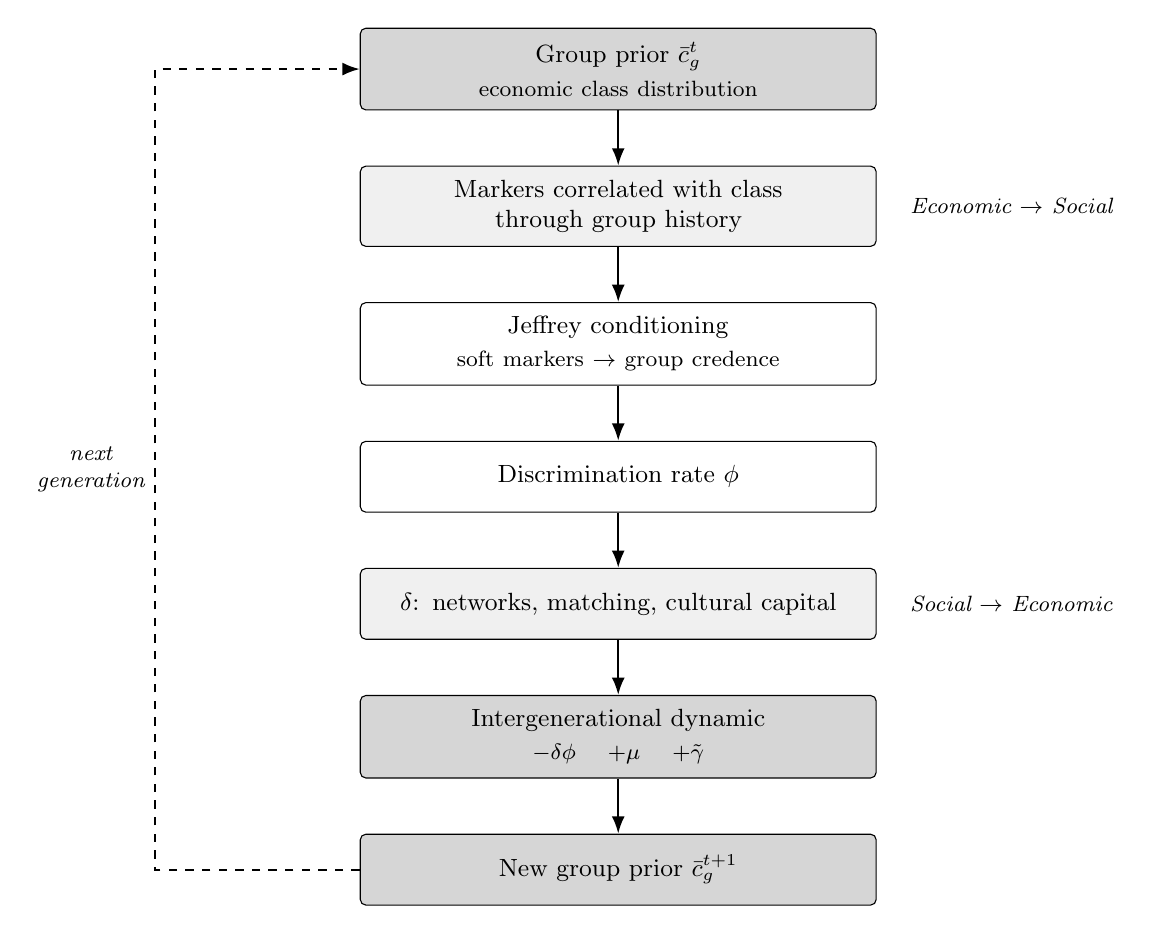
\begin{tikzpicture}[
  node distance=7mm,
  box/.style={rectangle, draw, rounded corners=2pt, align=center, inner sep=5pt, minimum height=9mm, font=\small, text width=62mm},
  econ/.style={box, fill=black!16},
  soc/.style={box, fill=black!6},
  infer/.style={box, fill=white},
  arr/.style={-{Latex[length=2.2mm]}, thick},
  feedback/.style={-{Latex[length=2.2mm]}, thick, dashed},
  ilabel/.style={font=\footnotesize\itshape}
]
\node[econ] (prior) {Group prior $\bar{c}_g^{t}$\\[1pt]{\footnotesize economic class distribution}};
\node[soc, below=of prior] (markers) {Markers correlated with class\\through group history};
\node[infer, below=of markers] (jeffrey) {Jeffrey conditioning\\[1pt]{\footnotesize soft markers $\to$ group credence}};
\node[infer, below=of jeffrey] (phi) {Discrimination rate $\phi$};
\node[soc, below=of phi] (delta) {$\delta$: networks, matching, cultural capital};
\node[econ, below=of delta] (dynamic) {Intergenerational dynamic\\[1pt]{\footnotesize $-\delta\phi$ \quad $+\mu$ \quad $+\tilde{\gamma}$}};
\node[econ, below=of dynamic] (newprior) {New group prior $\bar{c}_g^{t+1}$};

\draw[arr] (prior) -- (markers);
\draw[arr] (markers) -- (jeffrey);
\draw[arr] (jeffrey) -- (phi);
\draw[arr] (phi) -- (delta);
\draw[arr] (delta) -- (dynamic);
\draw[arr] (dynamic) -- (newprior);

\node[ilabel, right=3mm of markers] {Economic $\rightarrow$ Social};
\node[ilabel, right=3mm of delta] {Social $\rightarrow$ Economic};

\draw[feedback] (newprior.west) -- ++(-2.6,0) |- (prior.west)
  node[pos=0.25, left, ilabel, align=center] {next\\generation};
\end{tikzpicture}
\caption{The coupled two-system loop across one generation.
Mid-grey nodes are economic-system states, light-grey nodes are
social-system states, white nodes are the inference mechanism. The
economic system sets the meaning of markers (top interaction); the
social system erodes the group's economic position (bottom
interaction). The dashed arrow closes the loop: the new group prior
is what the next generation's markers are read against.}
\label{fig:loop}
\end{figure}

\subsection{Social engagement and the closure equilibrium}
\label{subsec:jeffrey}
\label{subsec:bilateral}
\label{subsec:interaction}
\label{sec:closure}

Jeffrey conditioning generalises Bayesian conditionalisation to evidence
that does not admit a likelihood function over the partition of interest
\citep{Jeffrey1965,Jeffrey2004}. The standard Bayesian update presupposes
a sharp evidence event $E$ with conditional probabilities $P(E \mid g_k)$
defined for each cell of the partition, yielding
$P(g_k \mid E) \propto P(E \mid g_k) P(g_k)$. When the agent's evidence is
a passage of experience that cannot be reduced to a proposition believed
with certainty---Jeffrey's founding example is observation of a coloured
cloth under poor light, leaving the observer with revised degrees of
belief over its possible colours but no proposition $E$ they have come
to believe with certainty \citep[\S 11.1]{Jeffrey1965}---the appropriate
revision is probability kinematics:
\begin{equation}
  P'(H) = \sum_{k=1}^{K} P(H \mid g_k) \cdot P'(g_k)
  \label{eq:kinematics}
\end{equation}
for any hypothesis $H$ outside the partition $\{g_1, \ldots, g_K\}$,
where the post-experience partition weights $P'(g_k)$ are produced
directly by the uncertain experience. The formula derives from the law
of total probability applied to the posterior, under the
\emph{invariance condition} $P'(H \mid g_k) = P(H \mid g_k)$ for all $k$
and $H$ \citep[\S\S 11.3, 11.6]{Jeffrey1965}: conditional probabilities
given each partition cell are preserved across the revision. Standard
Bayesian conditionalisation is the limiting case in which the partition
weights concentrate on a single cell \citep[\S 11.5]{Jeffrey1965}. The
rule has an axiomatic foundation in \citet{DiaconisZabell1982}.

In our setting the hypothesis of interest is class $c$ and the partition
is group membership $\{g_1, \ldots, g_K\}$, so the within-group
conditional distributions $F_{g_k} = P(c \mid g_k)$ play the role of the
invariant conditionals, and the kinematics formula specialises as
follows. Agent $j$ observes soft marker $m_i$. This shifts $j$'s
distribution over group membership from $P(g_k)$ to $P'(g_k)$ without
determining which group $i$ belongs to. Under
\textbf{Jeffrey conditioning}:
\begin{equation}
  P'(c) = \sum_{k=1}^{K} F_{g_k} \cdot P'(g_k)
  \label{eq:jeffrey}
\end{equation}

The revision $P \to P'$ is driven by the reassigned partition
weights $P'(g_k)$: the observer's experience of the marker shifts
probability mass across groups without specifying a generative model
$P(m \mid g_k)$ for how markers are produced by group membership.
Standard Bayesian updating requires such a likelihood function;
Jeffrey conditioning does not. This is not merely a technical
absence. The kinematics formula is the natural form updating takes
when evidence bears directly on a belief held with less
certainty---here, the partition weights $P(g_k)$ governing which
group a particular stranger belongs to---without bearing directly on
a belief held with more certainty: the within-group economic
distributions $F_{g_k}$, which the agent infers from aggregate
historical and statistical knowledge over many individuals.
\citet{Jeffrey2004} develops this picture explicitly: an agent's
beliefs form a chain held at varying strengths, and incoming
evidence redistributes probability across that chain in proportion
to where it bears.

\begin{example}[Jeffrey versus Bayes on a single counter-example]
\label{ex:jeffrey-bayes}
An observer meets a stranger at a professional gathering, with prior
credence split evenly between two groups, $P(g_A) = P(g_B) = 0.5$. The
observer's group priors---the group-level probabilities of high economic
class---are $\bar{c}_{g_A} = 0.7$ and $\bar{c}_{g_B} = 0.3$. Before any
signal, the expected probability that the stranger is high-class is
$0.5 \times 0.7 + 0.5 \times 0.3 = 0.50$.

The stranger speaks, and a soft marker (accent) shifts the observer's
group credence to $P'(g_A) = 0.2$, $P'(g_B) = 0.8$. The marker carries
no likelihood $P(m \mid \text{class})$: it is informative about group,
not directly about class. Jeffrey conditioning therefore holds the group
priors $\bar{c}_{g_k}$ fixed and revises only the group weights, giving
an updated class expectation of $0.2 \times 0.7 + 0.8 \times 0.3 = 0.38$.
The stranger's inferred standing falls from $0.50$ to $0.38$---not
because the accent revealed anything about this individual's income, but
because it reweighted the groups whose priors the observer already held.

Now suppose the stranger is in fact high-class. Under Jeffrey
conditioning the observer reclassifies the individual---attributing them
to $g_A$, or treating them as an exception within $g_B$---while
$\bar{c}_{g_B}$ is untouched: the next member of $g_B$ is met with the
same prior $0.3$. Under standard Bayesian updating on the same encounter,
observing a high-class member of $g_B$ raises the posterior
$\bar{c}_{g_B}$ above $0.3$; repeated such encounters drive it toward its
true value and the stereotype erodes. This divergence is the entire
mechanism: the same counter-example that a Bayesian absorbs into the
group \emph{belief}, the Jeffrey updater absorbs into the group
\emph{assignment}, leaving the belief intact.
\end{example}

\textbf{Rigidity condition} (Jeffrey's invariance, applied to
within-group conditionals)\textbf{.} What
Example~\ref{ex:jeffrey-bayes} illustrated is a general property of
the kinematics: the conditional probabilities $F_{g_k}$ are held
fixed during the Jeffrey revision. The substantive content of this
condition is epistemic: the agent's beliefs about the within-group
economic distribution $F_{g_k}$, built up over many observations and
statistical regularities, are held far more firmly than her beliefs
about an individual stranger's group membership, which a single
soft marker observation directly informs. The marker moves the
weaker belief without disturbing the stronger one. The kinematics
formula~(\ref{eq:jeffrey}) is the appropriate limiting form in this
regime---partition weights $P(g_k)$ far less certain than
within-group conditionals $F_{g_k}$---so updating concentrates on
the former. Consequence: an individual counter-example shifts
$P'(g_k)$---the individual is attributed to a different group---but
does \emph{not} update $F_g$. This is the formal expression of the
``exception to the rule'' phenomenon and stereotype persistence.
The condition is epistemic, not motivational: it concerns how
soft-marker evidence flows through the agent's hierarchy of beliefs,
not what the agent prefers. Whether agents additionally hold direct
preferences over group membership---taste-based discrimination in
the sense of \citet{Becker1957}---is a separate question that the
model does not turn on; the inference channel operates either way.

The information structure is bilateral and reflexive. Both agents
update simultaneously. Agent $i$'s self-belief is revised through
observing $j$'s consumption signals:
\begin{equation}
  Q_i'(c_i) = \sum_{k} Q_i(c_i \mid c_j = c_k) \cdot R_i'(c_k)
  \label{eq:bilateral}
\end{equation}
where $R_i'(c_k)$ is $i$'s Jeffrey-revised belief about $j$'s class
after observing $j$'s consumption bundle.

Three consequences follow from the bilateral Jeffrey structure.
First, exclusion suppresses aspirations and self-perception, not
just economic opportunities: the self-belief revision
(\ref{eq:bilateral}) downweights $i$'s own class assessment when
encountered agents signal exclusion (\emph{self-signalling and
aspiration formation}). Second, because the Jeffrey revision
(\ref{eq:jeffrey}) is driven by the partition weights $P'(g_k)$ and
these are produced by observed markers, agent $i$ has incentive to
manipulate markers to shift $P'(g_k)$ in $j$'s revision---the social
analogue of \citet{Spence1973}'s signalling model
(\emph{endogenous signal production}; Appendix~\ref{app:veblen}).
Third, the rigidity condition prevents the within-group
distributions $F_g$ from updating in response to individual
encounters, so excluded agents accumulate worse information about
economic opportunities than they otherwise would; the closure trap,
derived formally in Section~\ref{subsec:intergenerational}, is also
an information trap (\emph{closure as epistemic trap}).

Beliefs about class translate into an engagement decision through a
utility function in which class distance acts as a friction:
\begin{equation}
  U(c_i, c_j) = v - \kappa \cdot d(c_i, c_j)
  \label{eq:utility}
\end{equation}
where $v > 0$ is baseline interaction value, $\kappa > 0$ is
incompatibility sensitivity, and $d(\cdot)$ is the class distance.
The baseline value $v$ is the payoff from engaging with an agent of
identical class ($d(c_i, c_j) = 0$): it represents the intrinsic
benefit of social contact when the interaction partner is perfectly
compatible, and is reduced linearly by class distance through the
sensitivity parameter $\kappa$.
The agent's outside option $\bar{u}$ is the reservation payoff from
declining to engage---the utility available from remaining within an
existing social network rather than interacting with the encountered
individual. The utility depends on class distance
alone; group membership $g$ does not enter as an argument of $U$.
The dependence on group, when it appears in the model, arises
entirely through the agent's belief about $c_i$, which is
Jeffrey-updated from the observed marker as in (\ref{eq:jeffrey}).

Expected utility under Jeffrey-updated posterior:
\begin{equation}
  \E[U \mid m_i] = v - \kappa \cdot \E[d(c_i, c_j) \mid m_i]
  \label{eq:exp-utility}
\end{equation}

Agent $j$ engages iff:
\begin{equation}
  \E[d(c_i, c_j) \mid m_i] \leq
  \frac{v - \bar{u}}{\kappa} \equiv \Delta^*(c_j)
  \label{eq:threshold}
\end{equation}

Under bilateral structure, engagement requires condition
(\ref{eq:threshold}) to hold for both agents simultaneously.

The framework above applies to any number of groups $K$ and any
soft marker space. To develop closed-form equilibrium dynamics and
connect markers to the engagement decision, we now specialise on
two dimensions.

\textbf{Two-group simplification.} For the remainder of the
analysis, we work with two groups $\G = \{g_1, g_2\}$ (host and
immigrant/out-group respectively). This is the simplest
non-trivial setting for the asymmetry that drives the model; the
analysis generalises to $K$ groups at the cost of notation.

\textbf{Marker salience.} The Jeffrey revision (\ref{eq:jeffrey})
reassigns probability mass across the partition $\{g_1, g_2\}$; we
parametrise the strength of that reassignment by a scalar
$s_g \in [0,1]$, the probability the observer attributes the
encountered individual to the out-group upon observing their
markers:
\begin{equation}
  P'(g_2 \mid m_i) \equiv s_g
  \label{eq:salience}
\end{equation}
Marker salience is a property of the \emph{marker--observer
interaction}, not an intrinsic property of the group. A South Asian
individual in England has high $s_g$ (phenotypic markers strongly
identify out-group membership); the same individual in South Asia
has $s_g \approx 0$. Mutable markers (accent, dress, consumption)
can be modified, reducing $s_g$ over time; immutable markers (skin
colour, facial structure) produce permanently high $s_g$.

Under this parametrisation, the expected class distance for an
agent $j$ with class $c_j$ encountering an individual whose markers
trigger salience $s_g$ decomposes into bias and variance
components. Writing $\sigma_{g_k}^2$ for the within-group variance
of class outcomes in group $g_k$ (defined in
Appendix~\ref{app:bernoulli}):
\begin{equation}
  \begin{aligned}
  \E[d(c_i, c_j) \mid m_i]
  &= P'(g_2 \mid m_i) \cdot D_2 + P'(g_1 \mid m_i) \cdot D_1 \\
  &= s_g \underbrace{\left[(\bar{c}_{g_2} - c_j)^2 + \sigma_{g_2}^2\right]}_{D_2}
  + (1 - s_g) \underbrace{\left[(\bar{c}_{g_1} - c_j)^2 + \sigma_{g_1}^2\right]}_{D_1}
  \end{aligned}
  \label{eq:Ed-salience}
\end{equation}
The first line is the standard expected-utility form---a sum of
conditional expected distances weighted by posterior probabilities;
the second uses the definition $s_g \equiv P'(g_2 \mid m_i)$ from
(\ref{eq:salience}) and the binary partition $P'(g_1 \mid m_i) = 1 -
s_g$ to express the same expectation in the marker-salience
shorthand used in the remainder of the paper.
$D_k = (\bar{c}_{g_k} - c_j)^2 + \sigma_{g_k}^2$ is the
expected squared distance under certain attribution to group $g_k$.\footnote{This is the standard bias--variance decomposition of expected squared loss: both the squared gap between $c_j$ and the group mean (bias) and the within-group dispersion (variance) enter the agent's expected utility. Variance enters mechanically rather than as a separate risk-aversion parameter---the agent maximises expected utility under a quadratic distance metric, and $\E[(c_i - c_j)^2 \mid g_k] = (\E[c_i \mid g_k] - c_j)^2 + \mathrm{Var}(c_i \mid g_k)$ by definition.}
The within-group variance term $\sigma_{g_k}^2$ matters in its own
right: even when the group mean is close to the agent's class,
within-group heterogeneity raises expected class distance and the
probability that the engagement threshold (\ref{eq:threshold}) is
violated.
When $s_g = 1$, the observer attributes the individual to the
out-group with certainty and the expression reduces to:
\begin{equation}
  \E[d(c_i, c_j) \mid g_2]
  = (\bar{c}_{g_2} - c_j)^2 + \sigma_{g_2}^2
  \label{eq:Ed-group}
\end{equation}
which is the workhorse expression of the model. When $s_g = 0$,
the markers are invisible and the observer treats the individual
as a member of the host group: no discrimination occurs regardless
of economic history.

The engagement threshold is violated when either the bias (class
distance between observer and group mean) or the within-group
heterogeneity, weighted by marker salience, is too
large. When the threshold (\ref{eq:threshold}) is violated, agent
$j$ declines to engage with $i$: this is the model's discrimination
event. The discrimination mechanism therefore has two governing
parameters corresponding to the spatial and temporal dimensions of
social observation.\footnote{\label{rem:spacetime}Every soft signal
that enters the model is either a spatial property of the individual
observable at the encounter or encodes temporal information
accumulated across the group's economic history. Consequently,
spatial interventions (reducing marker visibility through assimilation
or ``passing'') and temporal interventions (raising the mobility
parameter $\gamma$ above its bifurcation threshold
$\gamma^*$ through mobility programmes) are categorically different
and cannot substitute for each other.} Marker salience $s_g$ is a
\emph{spatial} property: it is determined by what the observer
perceives at the point of encounter---phenotype, dress, accent, body
language---and governs \emph{whether} the Jeffrey revision fires and
how strongly. The group prior $\bar{c}_g$ is a \emph{temporal}
property: it is the sediment of the group's economic history across
generations and governs \emph{what} the Jeffrey revision maps to
once it fires. The model's central result---that sustained
discrimination requires both channels to be active---can be restated:
sustained discrimination requires both spatial identifiability
($s_g > 0$) and temporal disadvantage ($\bar{c}_g <
\bar{c}_g^{\mathrm{mid}}$).

Bilateral engagement decisions aggregate into a population-level
dynamic through two steps. First, within generation $t$, each
encounter between an in-group agent and a group-$g$ individual
produces engagement or refusal according to (\ref{eq:threshold});
the discrimination rate $\phi^t$ is the population fraction of
such encounters in which the threshold is violated. Second,
$\phi^t$ feeds back into the next generation's group prior
$\bar{c}_g^{t+1}$ through three economic channels: exclusion
(refused engagements deprive group $g$ of class-improving social
contact and erode the prior), natural convergence (an exogenous
intergenerational tendency toward the population mean), and
intergenerational mobility (within-group regression to the mean,
which depends on the current heterogeneity of group outcomes).
Combining these channels, the group prior evolves as:
\begin{equation}
  \bar{c}_g^{t+1} =
  \underbrace{\bar{c}_g^t(1 - \delta \phi^t)}_{\text{exclusion erodes prior}}
  + \underbrace{\mu(1 - \bar{c}_g^t)}_{\text{natural convergence}}
  + \underbrace{\tilde{\gamma}\,\bar{c}_g^t(1-\bar{c}_g^t)}_{\text{mobility from within-group heterogeneity}}
  \label{eq:dynamic}
\end{equation}
where $\delta > 0$ is the economic cost of social exclusion per unit
of discrimination, $\mu \in (0,1)$ is the exogenous intergenerational
convergence rate, and $\gamma \in (0,1)$ is the intergenerational
mobility parameter governing regression to the group mean.

The parameter $\delta$ is a reduced form. Social exclusion translates
into economic erosion through at least three channels that the model
does not separately distinguish: the matching market, where exclusion
from elite social spaces reduces the probability of assortative
pairing with higher-class partners
\citep{ColeMailathPostlewaite1992}; cultural capital, where
participation in social environments builds dispositions---accent,
self-presentation, institutional fluency---with direct economic
returns \citep{Bourdieu1984}; and information networks, where
informal social contact mediates access to economic opportunities
such as job referrals, mentorship, and business formation
\citep{Granovetter1973}. Each channel converts social exclusion into
a drag on intergenerational economic position; $\delta$ captures
their aggregate effect without requiring the model to specify which
dominates.

To anchor the decomposition: think of a group's economic position
passing across generations. Three channels operate. The
exclusion-erosion term $\bar{c}_g^t(1 - \delta \phi^t)$ carries
forward the parents' position but discounts it by the discrimination
rate---every economic interaction prevented by discrimination
reduces the group's economic position over time. The
natural-convergence term $\mu(1 - \bar{c}_g^t)$ is a rising tide
that lifts the group regardless of its current position---productivity
gains, public-good expansion, baseline improvement independent of
group status. The mobility term $\tilde{\gamma}\,\bar{c}_g^t(1-\bar{c}_g^t)$
captures intergenerational regression to the group mean---children
of high-class parents within the group may fall, children of
low-class parents may rise---and is largest at intermediate $\bar{c}_g$
where the within-group population is most heterogeneous. The
decomposition's analytical power is what it implies for two groups
in the same economy: identical $\mu$, identical heterogeneity,
identical mobility parameter $\tilde{\gamma}$---yet if only one of
them faces $s_g > 0$, the trajectories diverge from generation $t$
onward through the discrimination rate $\phi^t$. These three
channels are precisely the components labelled in the
intergenerational-dynamic node of Figure~\ref{fig:loop}.

To express (\ref{eq:dynamic}) as a one-dimensional dynamic in
$\bar{c}_g^t$, two further specifications are required: the closed
form of the mobility term, and the closed form of the discrimination
rate $\phi^t$.

Under the Beta--De~Finetti structure
(Appendix~\ref{app:bernoulli}), the within-group variance is
$\sigma_g^2 = \bar{c}_g(1-\bar{c}_g)/(1+\nu)$, where $\nu > 0$ is
the within-group concentration parameter, so the mobility term
becomes $\tilde{\gamma}\,\bar{c}_g(1-\bar{c}_g)$ where
$\tilde{\gamma} = \gamma/(1+\nu)$ is the effective mobility
parameter. This term is maximised at
group prior $\bar{c}_g = 1/2$ (maximum heterogeneity) and vanishes at $\bar{c}_g = 0$
and $\bar{c}_g = 1$ (homogeneous group). It captures
intergenerational regression to the group mean: children of
high-class families face some probability of downward mobility, and
children of low-class families have some chance of upward mobility.

The mobility parameter $\gamma$ is taken as exogenous: it captures
within-group variance arising from talent, effort, and wealth shocks,
independent of the group's social position. This is a significant
simplifying assumption. If $\gamma$ were endogenous---decreasing in
the discrimination rate $\phi$ through reduced access to education,
mentorship, and opportunity networks---the closure trap would be more
severe and the bifurcation threshold $\gamma^*$ harder to reach. The
assumption does not affect the rigidity condition, the tokenism or
shadow-market results, or the irreducibility of informational welfare
loss, all of which are independent of $\gamma$. It does affect the
bifurcation result quantitatively: the stated $\gamma^*$ understates
the required mobility intervention, because in the trap basin
$\gamma$ would itself be endogenously depressed, making the threshold
a moving target that recedes as discrimination intensifies. The
results that follow therefore hold a fortiori under endogenous
mobility, but the policy implication is sharper than stated: the
required intervention is larger than the exogenous model suggests.

\subsection{Intergenerational dynamics and the closure equilibrium}
\label{subsec:dynamics}

We now reduce the intergenerational dynamic (\ref{eq:dynamic}) to a
one-dimensional discrete dynamical system in the group prior
$\bar{c}_g$ and characterise its steady states. The analysis uses
only elementary properties of such systems---fixed points, the
slope condition for local stability, and the saddle-node
bifurcation; a reader unfamiliar with these may consult
\citet{Galor2007} for fixed points and stability and
\citet{MedioLines2001} for bifurcation analysis. A fixed point is a
group prior that reproduces itself from one generation to the next;
it is locally stable when the map's slope there is less than one in
absolute value, so that nearby trajectories are drawn toward it. The
substantive content is that the system admits more than one stable
fixed point, and that which one a group reaches depends on its
history.

The discrimination rate $\phi^t = s_g \cdot F(\bar{c}_g^t)$ is
determined by the engagement threshold (\ref{eq:threshold}),
modulated by marker salience $s_g$
(Proposition~\ref{prop:salience}), where $F: [0,1] \to [0,1]$ is
the group-level discrimination rate function induced by the
threshold: when $s_g = 0$, markers are
invisible and no discrimination fires. The composed map is:
\begin{equation}
  \mathcal{H}(\bar{c}_g;\, s_g) = \mu + \bar{c}_g(1 - \mu + \tilde{\gamma}
  - s_g\,\delta\, F(\bar{c}_g))
  - \tilde{\gamma}\,\bar{c}_g^2
  \label{eq:composed}
\end{equation}

The boundary conditions $\mathcal{H}(0; s_g) = \mu > 0$ and
$\mathcal{H}(1; s_g) = 1$ hold for all marker salience $s_g$, since $F(1) = 0$ and the
$\tilde{\gamma}$ terms cancel at $\bar{c}_g = 1$.

The map $\mathcal{H}$ governs the intergenerational evolution of the group
prior: $\bar{c}_g^{t+1} = \mathcal{H}(\bar{c}_g^t; s_g)$, so iterating $\mathcal{H}$
traces the group's class trajectory across generations. Fixed
points $\bar{c}_g^* = \mathcal{H}(\bar{c}_g^*; s_g)$ are self-reproducing
states---generations whose class profile replicates itself across
the intergenerational map. Whether such a state is desirable
depends on where it sits in $[0,1]$: a fixed point near
$\bar{c}_g = 1$ is integration, a fixed point near $\bar{c}_g = 0$
is exclusion. The three terms in $\mathcal{H}$ compete to determine which
arise as steady states. Mean-reversion ($\mu$) pulls upward from
low priors; the exclusion drag $-s_g \delta F(\bar{c}_g)$
generated by the engagement threshold pulls downward when
discrimination fires; and mobility, contained in the
$\tilde{\gamma}\,\bar{c}_g(1 - \bar{c}_g)$ term, generates
regression to the group mean. When exclusion dominates at low
$\bar{c}_g$, $\mathcal{H}$ dips below the 45-degree line and a second stable
fixed point appears at the low end. This is the closure trap,
which we now formalise.

\begin{definition}[Closure Equilibrium]
\label{def:closure}
A closure equilibrium is a fixed point $(\phi^*, \bar{c}_g^*)$ of the
composed map such that beliefs are consistent with outcomes and
outcomes with beliefs.
\end{definition}

\begin{proposition}[Class closure in a homogeneous society]
\label{prop:class-closure}
In the single-group model ($\G = \{g_1\}$), markers signal class
position directly. For sufficiently small $\gamma$ and sufficiently
large $\delta$, the map $\mathcal{H}$ has at least two stable fixed points
$\bar{c}_g^{\mathrm{low}} < \bar{c}_g^{\mathrm{high}} = 1$, separated by an unstable tipping point
$\bar{c}_g^{\mathrm{mid}}$. The low fixed point constitutes a
within-group class closure trap: a segment of the population is
permanently excluded from high-class social spaces across
generations, without any inter-group dynamic.
\end{proposition}

\begin{proof}[Proof sketch]
Define $\Psi(\bar{c}_g) = \mathcal{H}(\bar{c}_g) - \bar{c}_g$. Then $\Psi(0) = \mu > 0$
and $\Psi(1) = 0$ (since $F(1) = 0$ and the $\tilde{\gamma}$ terms cancel).
For sufficiently large $\delta$ and small $\gamma$, the exclusion
drag dominates at low $\bar{c}_g$, producing an S-shape in
$\mathcal{H}$ that forces $\Psi$ below zero on an interval in
$(0,1)$. By continuity and the Intermediate Value Theorem, $\Psi$
therefore has two interior roots: one where $\Psi$ crosses from
positive to negative ($\bar{c}_g^{\mathrm{low}}$, stable) and one
where it crosses back ($\bar{c}_g^{\mathrm{mid}}$, unstable), in
addition to the boundary root at $\bar{c}_g = 1$. Local stability
follows from $|\mathcal{H}'(\bar{c}_g^{\mathrm{low}})| < 1$ and
instability from $\mathcal{H}'(\bar{c}_g^{\mathrm{mid}}) > 1$.
Path dependence follows from $\mathcal{H}' > 0$ on the relevant
intervals, which ensures monotonicity of orbits on each side of
$\bar{c}_g^{\mathrm{mid}}$ \citep[see][ch.~1]{Galor2007}. \qed
\end{proof}

\begin{figure}[ht]
\centering
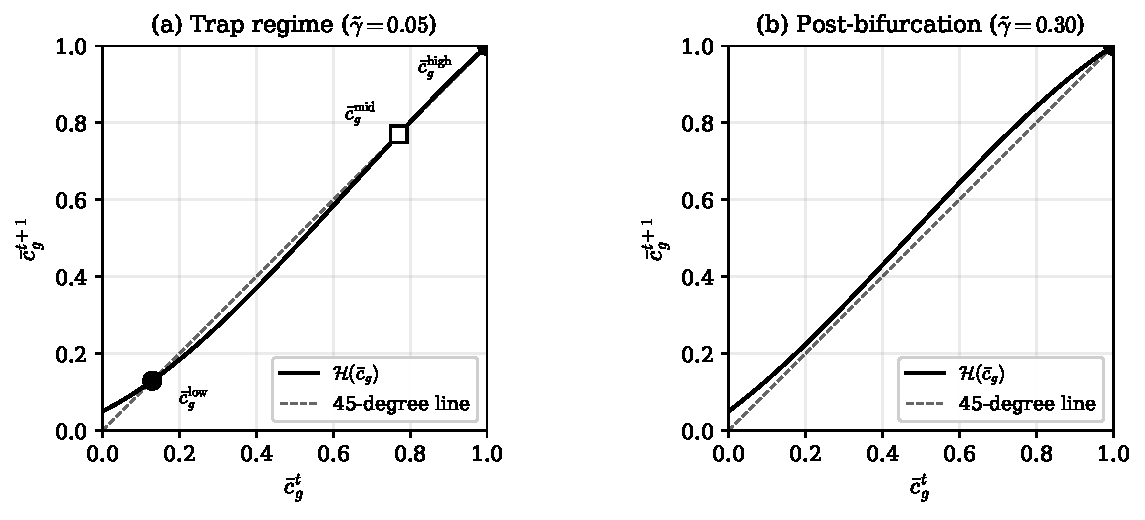
\includegraphics[width=\textwidth]{figures/Fig1}
\caption{Composed map $\mathcal{H}(\bar{c}_g;\, s_g)$ plotted against
the 45-degree line. Stable fixed points are shown as filled circles,
the unstable tipping point as an open square. Panel (a): trap regime,
three fixed points $\bar{c}_g^{\mathrm{low}}$,
$\bar{c}_g^{\mathrm{mid}}$, $\bar{c}_g^{\mathrm{high}} = 1$. Panel (b):
post-bifurcation, the unique stable fixed point is $\bar{c}_g = 1$.
Illustrative functional form $F(\bar{c}_g) = (1 - \bar{c}_g)^2$ and
parameters $\mu = 0.05$, $\delta = 0.5$, $s_g = 1$.}
\label{fig:closure-map}
\end{figure}

\subsection{Comparative statics and the mobility threshold}
\label{subsec:intergenerational}

We now characterise the individual-level mechanics of the
discrimination mechanism. The four results that follow describe how
an agent's own economic class, education, and the group's economic
history shape the engagement decision, and how the Jeffrey framework
produces graded rather than binary discrimination.

\begin{proposition}[Income effect]
\label{prop:income}
Higher own economic class increases the expected class proximity to
other high-class agents, expanding the engagement set:
$\partial \E[d(c_i, c_j)\mid g]/\partial c_j = -2(\bar{c}_g - c_j) < 0$ when $c_j < \bar{c}_g$.
\end{proposition}

\begin{proposition}[Education effect]
\label{prop:education}
Higher own education increases precision of marker-to-group mapping,
increasing responsiveness of $P'(g_k)$ to individual information and
reducing weight on group prior $F_g$.
\end{proposition}

\begin{proposition}[Economic history effect]
\label{prop:history}
Lower $\bar{c}_g$ generates higher posterior expected
incompatibility for any given marker, pushing more potential partners
below the engagement threshold:
$\partial \E[d(c_i, c_j)\mid g]/\partial \bar{c}_g = 2(\bar{c}_g - c_j) < 0$ when
$c_j > \bar{c}_g$.
\end{proposition}

\begin{proposition}[Graded discrimination]
\label{prop:graded}
The Jeffrey framework predicts continuous variation in avoidance with
marker ambiguity. A faint accent produces less avoidance than a
strong one. $\E[d(c_i, c_j)]$ is quadratic in $\bar{c}_g$
($\partial^2 \E/\partial \bar{c}_g^2 = 2 > 0$), distinguishing the model
from Phelps--Arrow's binary response to hard group membership.
\end{proposition}

We now turn to the role of marker salience---the spatial dimension
of the model---and the policy instrument of forced suppression. The
two results that follow establish how salience interacts with
economic history to determine whether discrimination is sustained or
extinguished, and what happens when the salience channel is
constrained by policy.

\begin{proposition}[Marker salience effect]
\label{prop:salience}
Higher marker salience amplifies expected incompatibility when the
out-group is economically disadvantaged:
\[
  \frac{\partial \E[d(c_i, c_j) \mid m_i]}{\partial s_g}
  = D_2 - D_1 > 0
  \quad \text{when } \bar{c}_{g_2} < \bar{c}_{g_1}.
\]
Two groups with identical economic histories $\bar{c}_g$ face
different closure dynamics if their marker salience differs. Marker
salience and economic history are jointly necessary for sustained
discrimination: $s_g = 0$ eliminates discrimination regardless of
$\bar{c}_g$, and $\bar{c}_{g_2} = \bar{c}_{g_1}$ eliminates
discrimination regardless of $s_g$.
\end{proposition}

\begin{proposition}[Forced marker suppression]
\label{prop:suppression}
Let $\lambda_s \in [0,1]$ be a policy instrument that caps effective
marker salience: $s_g^{\mathrm{eff}} = \min(s_g,\, \lambda_s)$.
When the cap binds ($\lambda_s < s_g$):
\begin{enumerate}[noitemsep]
  \item The discrimination rate falls:
  $F(\bar{c}_g,\, \lambda_s) < F(\bar{c}_g,\, s_g)$.
  \item The mobility threshold falls:
  $\tilde{\gamma}^*(\lambda_s) < \tilde{\gamma}^*(s_g)$.
  \item The shadow information value of the remaining unsuppressed
  markers rises: $\partial \Omega_j / \partial \lambda_s < 0$
  conditional on $\lambda_s < s_g$. Suppressing one class of markers
  raises the discriminatory return to those that remain.\footnote{The
  model uses a single aggregate $s_g$. The substitution claim is a
  structural argument: if the model were extended to a vector
  $\mathbf{s} = (s_1, \ldots, s_K)$ with channel-specific
  suppression, partial suppression on channel $k$ would raise
  the shadow return to unsuppressed channels. A formal
  multi-channel extension is left for future work.} Partial
  suppression produces marker reallocation, not elimination.
  \item When suppression is lifted ($\lambda_s \to s_g$), the
  equilibrium snaps to the state the unsuppressed system would
  have converged to. If $\bar{c}_g$ has not crossed
  $\bar{c}_g^{\mathrm{mid}}$ during the suppression period, the
  closure trap re-emerges immediately. The speed of
  re-stratification is proportional to the gap
  $s_g - \lambda_s$.
\end{enumerate}
\end{proposition}

The preceding comparative statics describe how individual-level
parameters and marker salience shape the discrimination rate within
a single generation. The remaining results address two deeper
questions. First, can the closure trap be eliminated permanently, or
is it a structural feature of the system for any positive marker
salience? Second, what happens when a second group enters the model
with its own economic history and marker salience profile, and what
trajectories do its members follow? The next four results answer
these in sequence: the saddle-node bifurcation
(Proposition~\ref{prop:bifurcation}) characterises the mobility
threshold above which the trap is eliminated; the salience-threshold
corollary (Corollary~\ref{cor:salience-threshold}) shows how
immutable markers raise the threshold; the outsider-group result
(Proposition~\ref{prop:enemy}) traces the integration trajectory of
a low-prior out-group; and the passing result
(Proposition~\ref{prop:passing}) shows that individual exit from
the visible group through marker suppression worsens the position
of those who remain.

\begin{proposition}[Mobility threshold and bifurcation]
\label{prop:bifurcation}
There exists $\gamma^* > 0$ such that:
\begin{enumerate}[noitemsep]
  \item If $\gamma < \gamma^*$: the closure trap persists (two stable
  fixed points).
  \item If $\gamma > \gamma^*$: the closure trap is eliminated
  (unique stable fixed point at $\bar{c}_g = 1$).
  \item At $\gamma = \gamma^*$: a saddle-node bifurcation \citep[see][ch.~4]{MedioLines2001}---the low
  fixed point and the tipping point collide and annihilate.
\end{enumerate}
\end{proposition}

\begin{proof}[Proof sketch]
At $\gamma = 0$, the closure trap exists
(Proposition~\ref{prop:class-closure}). As the mobility parameter $\gamma$ increases, the
mobility term raises $\mathcal{H}(\bar{c}_g)$ in the interior, shrinking
the region where $\Psi < 0$. At $\gamma = \gamma^*$, the region
vanishes: the low fixed point and the tipping point merge,
$\mathcal{H}'(\bar{c}_g^*) = 1$, and the system undergoes a saddle-node
bifurcation. For $\gamma > \gamma^*$, $\Psi > 0$ on all of $(0,1)$
and the only fixed point is $\bar{c}_g = 1$. The exact $\tilde{\gamma}^*$ is
found numerically by solving the bifurcation system
$\{\mathcal{H}(\bar{c}_g) = \bar{c}_g,\; \mathcal{H}'(\bar{c}_g) = 1\}$ jointly.
\qed
\end{proof}

\begin{figure}[ht]
\centering
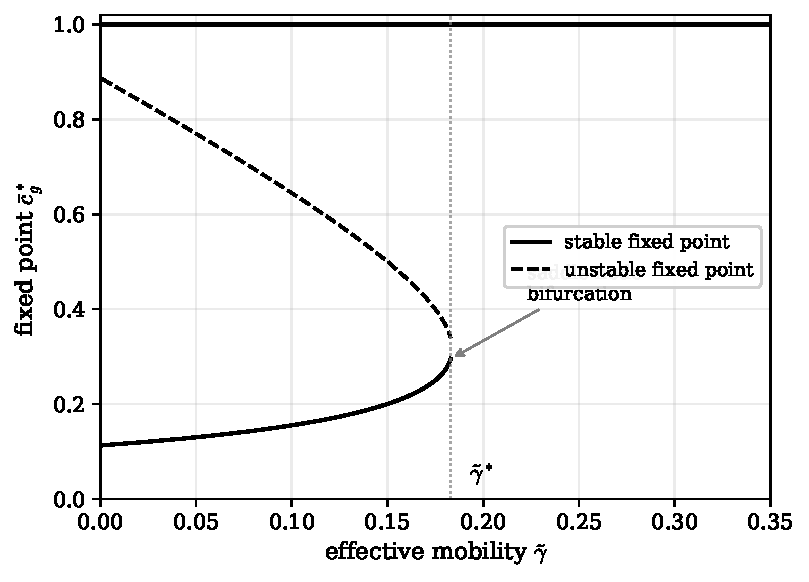
\includegraphics[width=0.7\textwidth]{figures/Fig2}
\caption{Bifurcation diagram of fixed points $\bar{c}_g^*$ against the
effective mobility parameter $\tilde{\gamma}$. Solid lines: stable fixed
points; dashed line: unstable tipping point. At
$\tilde{\gamma} = \tilde{\gamma}^*$ the low fixed point and the tipping
point collide and annihilate (saddle-node bifurcation), and the
closure trap is eliminated. Illustrative functional form
$F(\bar{c}_g) = (1 - \bar{c}_g)^2$ and parameters $\mu = 0.05$,
$\delta = 0.5$, $s_g = 1$.}
\label{fig:bifurcation}
\end{figure}

The intergenerational persistence of class position near the
bifurcation is characterised in Appendix~\ref{app:Tstar}.

\begin{corollary}[Marker salience raises the mobility threshold]
\label{cor:salience-threshold}
The critical mobility threshold $\tilde{\gamma}^*$ is strictly
increasing in marker salience:
$\partial \tilde{\gamma}^* / \partial s_g > 0$. At $s_g = 0$,
$\tilde{\gamma}^* = 0$ and no closure trap exists for any positive
mobility rate. At $s_g = 1$, $\tilde{\gamma}^*$ attains its maximum,
recovering the base-model threshold. Consequently, groups with
immutable markers (high $s_g$) require strictly higher
intergenerational mobility to escape the closure trap than groups
with mutable markers (low $s_g$), even when starting from identical
economic positions.
\end{corollary}

\begin{proof}[Proof sketch]
The composed map $\mathcal{H}(\bar{c}_g;\, s_g)$ is decreasing in marker salience $s_g$ on the
interior of $[0,1]$ (since $\partial G/\partial s_g = -\delta\phi
\bar{c}_g < 0$). A higher $s_g$ lowers $\mathcal{H}$ in the interior, deepening
the region where $\Psi < 0$ and requiring higher $\tilde{\gamma}$ to
restore $\Psi \geq 0$ everywhere. At $s_g = 0$, the discrimination
channel is fully shut off ($\phi^t = 0$ for all $t$), so
$\mathcal{H}(\bar{c}_g;\, 0) = \mu + \bar{c}_g(1 - \mu + \tilde{\gamma}) -
\tilde{\gamma}\bar{c}_g^2$, which satisfies $\Psi \geq 0$ for all
$\tilde{\gamma} \geq 0$. Numerical verification confirms strict
monotonicity across the full range of $s_g$. \qed
\end{proof}

\begin{definition}[Outsider group]
Group $g_2$ is an outsider group relative to host group $g_1$ if
$\bar{c}_{g_2}^0 < \bar{c}_g^{\mathrm{mid}}$---their prior starts
in the high-discrimination basin.
\end{definition}

The outsider group's integration trajectory depends on two dimensions:
economic history ($\bar{c}_{g_2}^0$) and marker salience ($s_g$).
A group with low $\bar{c}_{g_2}^0$ but also low $s_g$---phenotypically
similar to the host, with mutable cultural markers---may escape
the trap rapidly because the discrimination channel fires weakly.
A group with comparable $\bar{c}_{g_2}^0$ but high marker salience $s_g$---visibly
distinct, with immutable phenotypic markers---faces a structurally
harder path. The Irish in England illustrate the former: despite a
history of famine, colonial extraction, and armed conflict,
phenotypic similarity ($s_g \approx 0.15$) meant the Jeffrey
revision fired weakly, and integration occurred within two
generations. Indian and Kenyan immigrants illustrate the latter:
comparable or better initial economic positions but high phenotypic
salience ($s_g \approx 0.9$) sustains the closure trap
indefinitely under the same mobility parameters.

\begin{proposition}[Outsider trap]
\label{prop:enemy}
If $g_2$ enters with $\bar{c}_{g_2}^0 < \bar{c}_g^{\mathrm{mid}}$
and $s_g$ sufficiently high that $\tilde{\gamma} <
\tilde{\gamma}^*(s_g)$, then $g_2$ converges to the
high-discrimination equilibrium $\bar{c}_g^{\mathrm{low}}(g_2)$ independently
of $g_1$'s trajectory, and $g_1$'s equilibrium is unaffected.
If $s_g$ is sufficiently low that $\tilde{\gamma} >
\tilde{\gamma}^*(s_g)$, the trap does not exist and $g_2$
converges to the integration equilibrium regardless of initial
economic position.
\end{proposition}

\begin{proposition}[Adverse selection through passing]
\label{prop:passing}
When individuals can reduce their personal marker salience $s_{g,i}$
at cost $\kappa(c_i)$ decreasing in class (higher-class individuals
find it easier to ``pass''), selective exit from the visible
out-group worsens the remaining group's prior:
\[
  \frac{\partial \bar{c}_g^{\mathrm{visible}}}
  {\partial (\mathrm{passing\ rate})} < 0.
\]
The individuals most able to pass---those with highest $c_i$ and
lowest natural $s_{g,i}$---are positively selected. Their departure
lowers the mean class of the visible group, which in turn raises
the discrimination rate $F(\bar{c}_g)$ against those who remain.
Individual compliance does not merely fail to improve the group
prior (the rigidity condition); it actively worsens it through
composition. The mimic man's escape harms those he leaves behind.
\end{proposition}

The embedding of the model in a one-parameter family, with the
standard-Bayesian benchmark recovered as $\rho \to 0$, is developed
in Appendix~\ref{app:loury}.

% =============================================================================
\subsection{Institutional aggregation: the platform channel}
\label{sec:platform}
% =============================================================================

The bilateral analysis has so far treated encounters as occurring
between individuals. In many real settings the environment in which
they occur is itself produced by a market actor: a restaurant
calibrates its atmosphere to attract preferred compositions, a
school sets admission criteria, a neighbourhood configures itself
through pricing and zoning. We use ``platform'' to denote any such
venue, neighbourhood, school, or institution that mediates
encounters through an atmosphere vector and an admission policy.

The bilateral mechanism locates the first source of persistence at
the individual level: the rigidity condition ensures that compliance
does not aggregate into group prior revision. The platform identifies
a second source, which operates at the institutional level and is
independent of the first: even if bilateral encounters did not
generate persistence, profit-maximising platforms acting on soft
signals would produce discriminatory compositions as an emergent
outcome.

Embedding bilateral Jeffrey updating within a platform produces
three results absent from the bilateral setting: a shadow
information market whose intensity rises with legal strictness
(Proposition~\ref{prop:shadow}); optimal platform exclusion of
stigmatised groups that relaxes into a tokenism equilibrium before
genuine integration is achieved
(Propositions~\ref{prop:exclusion}--\ref{prop:tokenism}); and a host
destabilisation channel through which inclusion of the out-group
can trigger closure dynamics within the host group
(Proposition~\ref{prop:spillover}). The welfare implications of
these platform results, together with those of the bilateral
mechanism, are analysed in Section~\ref{sec:welfare}.

For a $g_1$ client $j$, experience utility at a venue with attendee
set $\A$ is:
\begin{equation}
  V_j(\A) = \alpha \cdot q + (1 - \alpha) \cdot S_j(\A)
  \label{eq:experience}
\end{equation}
where $q$ is objective quality, $\alpha \in (0,1)$ is the weight on
objective vs.\ social quality, and:
\begin{equation}
  S_j(\A) = \frac{1}{|\A|} \sum_{i \in \A,\, i \neq j}
  \E_j[c_i \mid m_i]
  \label{eq:social-quality}
\end{equation}

$S_j(\A)$ is a function of \emph{beliefs}, not facts.


The platform produces atmosphere vector
$\mathbf{a}$ (pricing, location, d\'{e}cor, dress code,
marketing language, music, staff manner) serving two functions.

\textbf{Function 1: Client self-selection.}
$\Pr(\text{visit} \mid c_j, \mathbf{a}) = h(c_j, \mathbf{a})$,
increasing in the match between $c_j$ and the class $\mathbf{a}$
signals.

\textbf{Function 2: Contextual modulation of Jeffrey updating.}
$P'(g_k \mid m_i, \mathbf{a}) \neq P'(g_k \mid m_i)$. A strong
high-class atmosphere acts as a contextual prior, resolving marker
ambiguity against the stigmatised group.

\begin{equation}
  \max_{\mathbf{a},\, \sigma} \quad
  \Pi(\mathbf{a}, \sigma) = \sum_{j \in \mathcal{D}(\mathbf{a})}
  \sigma(m_j) \cdot W_j(\mathbf{a}, \sigma) - C(\mathbf{a})
  \label{eq:platform-opt}
\end{equation}
where $\Pi$ is platform profit, $\mathcal{D}(\mathbf{a})$ is the
self-selecting set,
$\sigma: \M \to [0,1]$ is the admission policy, $W_j$ is willingness
to pay, and $C(\mathbf{a})$ is cost.

\textbf{Legal constraint:} $\sigma$ cannot be an explicit function of
group membership $g$. But $\sigma$ may depend on markers $m$, which
are correlated with $g$. Result: \emph{informationally mediated,
legally invisible discrimination}.

\begin{proposition}[Shadow market intensity]
\label{prop:shadow}
The shadow information value $\Omega_j$ satisfies:
\begin{enumerate}[noitemsep]
  \item $\Omega_j$ is decreasing in $\bar{c}_g$ for $\bar{c}_g < 1/2$:
  groups with worse economic histories generate higher shadow market
  intensity.
  \item $\partial \Omega_j / \partial (1-\alpha) > 0$: clients who
  weight social quality more invest more in shadow information.
  \item $\partial \Omega_j / \partial \lambda > 0$ where $\lambda$
  indexes legal strictness: tighter anti-discrimination law raises
  the return to shadow information. The mechanism: the law constrains
  formal screening but leaves shadow cues unconstrained, degrading
  the uninformed fallback while preserving the informed outcome.
  \item $\partial \Omega_j / \partial s_g > 0$: higher marker
  salience raises shadow market intensity, because visible markers
  make group attribution easier and therefore the informational
  advantage of knowing the ``right'' venues more valuable.
\end{enumerate}
\end{proposition}

\begin{proposition}[Platform exclusion of outsider group]
\label{prop:exclusion}
At the outsider group's entry prior $\bar{c}_{g_2}^0$, the platform
optimally excludes $g_2$ entirely:
$\sigma^*(m) = 0$ for all $m \in \M_{g_2}$.
\end{proposition}

\begin{proof}[Proof sketch]
The platform's first-order condition with respect to
$\sigma(m)$ for $m \in \M_{g_2}$ decomposes into two terms. The
direct revenue effect is the marginal willingness-to-pay $W(g_2)$ of
an admitted $g_2$ member. The composition externality is the
aggregated drop in social-quality perception across the $n_{g_1}$
host clients on the platform, weighted by $(1 - \alpha)$ from
equation~(\ref{eq:experience}): admitting one additional $g_2$
member shifts each host's $S_j(\mathcal{A})$ by
$(\bar{c}_{g_2} - \bar{c}_{g_1})/|\mathcal{A}| < 0$. The net
marginal profit is therefore
\[
  \frac{\partial \Pi}{\partial \sigma(m)} \;=\;
  W(g_2) \;+\; n_{g_1} (1 - \alpha)
  \cdot \frac{\bar{c}_{g_2} - \bar{c}_{g_1}}{|\mathcal{A}|}.
\]
At the entry prior $\bar{c}_{g_2}^0$, the gap
$\bar{c}_{g_1} - \bar{c}_{g_2}^0$ is large and $W(g_2)$ is bounded
above by the willingness-to-pay of a low-class admittee. The
externality term dominates and the derivative is negative, so the
platform's optimum is the corner $\sigma^*(m) = 0$.
\qed
\end{proof}

\begin{proposition}[Partial inclusion equilibrium]
\label{prop:tokenism}
The platform exclusion threshold $\bar{c}_g^{\mathrm{excl}}$ satisfies
$\bar{c}_g^{\mathrm{excl}} < \bar{c}_g^{\mathrm{mid}}$: the platform begins
admitting $g_2$ members \emph{before} they have escaped the
high-discrimination basin, creating a partial inclusion zone
$[\bar{c}_g^{\mathrm{excl}}, \bar{c}_g^{\mathrm{mid}}]$ in which $g_2$ has
platform access but not social integration.
\end{proposition}

\begin{proof}[Proof sketch]
The exclusion threshold $\bar{c}_g^{\mathrm{excl}}$ is the value of
$\bar{c}_{g_2}$ at which the platform's FOC (proof of
Proposition~\ref{prop:exclusion}) just balances:
\[
  W(g_2) \;=\; n_{g_1} (1 - \alpha)
  \cdot \frac{\bar{c}_{g_1} - \bar{c}_g^{\mathrm{excl}}}{|\mathcal{A}|}
\]
which is continuous in $\bar{c}_{g_2}$ through both $W(g_2)$ (rising
with $g_2$'s class) and the externality (shrinking as the gap
$\bar{c}_{g_1} - \bar{c}_{g_2}$ closes). The social tipping point
$\bar{c}_g^{\mathrm{mid}}$, by contrast, is determined by the
aggregate discrimination rate $F(\bar{c}_g)$ crossing the level at
which the closure basin disappears
(Proposition~\ref{prop:class-closure}); it is a property of the
system-wide intergenerational dynamic
in equation~(\ref{eq:dynamic}), not of the platform's marginal
calculation. Because the platform optimises against the local
average class signal inside the platform while
$\bar{c}_g^{\mathrm{mid}}$ depends on the global discrimination
rate, the two thresholds are determined by structurally different
objects, and the platform's FOC balances at a $\bar{c}_g$ strictly
below the social tipping point. \qed
\end{proof}

This equilibrium is the structural counterpart of what is
colloquially called tokenism: the platform admits members of the
stigmatised group before social integration is achieved, producing
visible inclusion without the underlying belief revision that
integration would require. The result emerges from the Jeffrey
mechanism and the platform's profit incentives, not from any
imputed intent on the platform's part. The admissions are not
cosmetic in their effect on the host group's social environment,
however: they alter the marginal composition of the platform and
can in turn destabilise the host equilibrium when the host group
itself is near its tipping point.

\begin{proposition}[Host destabilisation]
\label{prop:spillover}
If $g_1$'s equilibrium prior $\bar{c}_{g_1}^*$ is close to
$\bar{c}_g^{\mathrm{mid}}$, the platform's admission of $g_2$ members
at $\bar{c}_g^{\mathrm{excl}}$ can push $g_1$ below its own tipping
point, triggering a class-closure episode within the host group. The
critical $g_2$ fraction $\rho_{\mathrm{crit}}$ is decreasing in the
spillover sensitivity parameter $\varepsilon$.
\end{proposition}

\begin{proof}[Proof sketch]
Admitting $g_2$ members at fraction $\rho$ on the platform lowers
the local average class signal observed by $g_1$ clients by
$\rho \cdot (\bar{c}_{g_1}^* - \bar{c}_{g_2}^{\mathrm{excl}})$. The
spillover sensitivity $\varepsilon \in (0, 1]$ measures the fraction
of this local shift that transmits to $g_1$'s effective system-wide
prior through repeated platform encounters:
$\bar{c}_{g_1}^{\mathrm{eff}} = \bar{c}_{g_1}^*
- \varepsilon \rho (\bar{c}_{g_1}^* - \bar{c}_{g_2}^{\mathrm{excl}})$.
The host group crosses its tipping point when
$\bar{c}_{g_1}^{\mathrm{eff}} = \bar{c}_g^{\mathrm{mid}}$, giving
\[
  \rho_{\mathrm{crit}}
  \;=\; \frac{\bar{c}_{g_1}^* - \bar{c}_g^{\mathrm{mid}}}
  {\varepsilon \cdot (\bar{c}_{g_1}^* - \bar{c}_{g_2}^{\mathrm{excl}})}
\]
whose derivative
$\partial \rho_{\mathrm{crit}} / \partial \varepsilon$ is strictly
negative when $\bar{c}_{g_1}^*$ exceeds both $\bar{c}_g^{\mathrm{mid}}$
and $\bar{c}_{g_2}^{\mathrm{excl}}$, the configuration of interest.
\qed
\end{proof}

The platform framework extends naturally to immigration. An
immigrant's assimilation trajectory is determined by the economic
tier at which initial social attachment occurs: the host population's
Jeffrey revision maps the immigrant's foreign marker bundle
$m_i^{\text{foreign}}$ onto an initial prior
$\bar{c}_g^{\text{init}}$ that depends on marker legibility within
the host's marker space $\M$, not on actual economic class at origin.
Immigrants with legible high-class markers access high-class
platforms from the outset; those with illegible markers enter the
closure trap from below regardless of origin class. This generates
two channels in host preferences over immigration composition: a
\emph{closure-sustainability channel} (high-income hosts accept
pre-sorted high-class immigrants who expand the high-income network
without disrupting stratification) and a \emph{competition channel}
(same-tier arrivals compete in labour and social spaces, cutting
against the first motive). Points-based immigration systems are
formally attempts to certify marker legibility in advance of social
contact, converting soft foreign markers into a hard administrative
signal---consistent with the empirical finding that such systems
produce faster assimilation trajectories. The same framework
predicts that within-ethnic differential treatment by class
markers---software engineers and taxi drivers of shared national
origin receiving categorically different host treatment
\citep{LeeZhou2015, Waters1999}---is a direct consequence of the
bilateral model, with the platform channel reinforcing it.

% =============================================================================
\section{Welfare analysis}
\label{sec:welfare}
% =============================================================================

This section synthesises the welfare implications of the bilateral
mechanism and the platform channel developed in
Section~\ref{sec:model}. The decomposition that follows distinguishes
four loss components; three of them are properties of the bilateral
closure trap, and one is specific to the platform extension.

We define social welfare $W$ as the population-aggregate expected
utility from social engagement, summed across encounters within a
generation and discounted across generations. The first-best welfare
$W^*$ is achieved when every mutually beneficial encounter takes
place, the Jeffrey rigidity condition is non-binding, and no shadow
information market is active. The total welfare loss
$\mathcal{L} = W^* - W^{\mathrm{eq}}$ decomposes into four
components by a telescoping construction across counterfactual
welfares (formal derivation given in the welfare addendum):
\begin{equation}
  \mathcal{L} \;=\;
  \mathcal{L}_{\text{alloc}} \;+\; \mathcal{L}_{\text{info}}
  \;+\; \mathcal{L}_{\text{dyn}} \;+\; \mathcal{L}_{\text{platform}}.
  \label{eq:welfare}
\end{equation}
$\mathcal{L}_{\text{alloc}}$ is the expected foregone surplus from
refused beneficial encounters; under the engagement
threshold~(\ref{eq:threshold}) this is $s_g \cdot F(\bar{c}_g)
\cdot \overline{\Delta U}$, the discrimination rate weighted by
average foregone surplus per blocked encounter.
$\mathcal{L}_{\text{info}}$ is the welfare gap between the Jeffrey
equilibrium and the counterfactual Bayesian equilibrium that would
obtain if the rigidity condition were removed, bounded below by
$\rho \cdot \mathrm{dKL}(F_g \,\Vert\, F_g^{\mathrm{Bayes}})$.
$\mathcal{L}_{\text{dyn}}$ is the discounted sum of allocative
losses across future generations attributable to the closure
dynamic in $\bar{c}_g$. $\mathcal{L}_{\text{platform}}$ is the
aggregate cost of the shadow information market,
$\int \Omega_j\, dj$.

Of these four components, the informational loss
$\mathcal{L}_{\text{info}}$ is the decisive one. The allocative,
dynamic, and platform losses can each in principle be targeted by an
instrument aimed at them; the informational loss cannot. It is the only
component that no instrument leaving the soft-signal structure intact
can remove, as the irreducibility result below
(Corollary~\ref{cor:irreducibility}) establishes, and it is in this
sense that the contact channel sets a floor on what any
contracting-channel remedy can achieve.

The welfare implications follow from comparing how each policy
instrument in the class $\Phi$ (instruments that leave the
soft-signal structure invariant) acts across these components.

\begin{proposition}[Welfare dominance of mobility above $\gamma^*$]
\label{prop:dominance}
Within the policy class $\Phi$, mobility programmes raising
$\gamma$ above $\gamma^*$ are uniquely welfare-dominant in the long
run: they eliminate $\mathcal{L}_{\mathrm{dyn}}$ permanently
through the saddle-node bifurcation
(Proposition~\ref{prop:bifurcation}), eliminate
$\mathcal{L}_{\mathrm{alloc}}$ at the integration steady state, and
do not amplify $\mathcal{L}_{\mathrm{platform}}$. No other
instrument in $\Phi$ achieves elimination on more than one
component. Anti-discrimination law on the formal-contracting side
addresses $\mathcal{L}_{\mathrm{alloc}}$ on that channel but
displaces activity into the informal contact channel, raising
$\mathcal{L}_{\mathrm{platform}}$ through the shadow-market effect
of Proposition~\ref{prop:shadow}; the net welfare effect is
ambiguous without empirical calibration of which component
dominates.
\end{proposition}

\begin{proof}[Proof sketch]
Above $\gamma^*$ the saddle-node bifurcation destroys the closure
basin: the unique stable fixed point is the integration steady
state $\bar{c}_g = 1$, at which $F(\bar{c}_g) = 0$ and the
discrimination rate $\phi$ is zero. Both $\mathcal{L}_{\text{alloc}}$
and $\mathcal{L}_{\text{dyn}}$ therefore vanish. The mobility
instrument operates on $\gamma$, which does not enter the
platform's shadow-information optimisation, so
$\mathcal{L}_{\text{platform}}$ is unchanged. For any alternative
instrument in $\Phi$: anti-discrimination law on the contracting
side reduces $\mathcal{L}_{\text{alloc}}$ on that channel but
raises $\mathcal{L}_{\text{platform}}$ via
Proposition~\ref{prop:shadow}; forced integration shifts a cohort
above $\bar{c}_g^{\mathrm{mid}}$ but does not eliminate the basin,
so $\mathcal{L}_{\text{dyn}}$ persists for subsequent cohorts;
platform regulation reduces $\mathcal{L}_{\text{platform}}$ only.
The set of components eliminated by mobility above $\gamma^*$ is
therefore a strict superset of what any alternative achieves.
\qed
\end{proof}

The dominance result establishes which instrument is welfare-best
within $\Phi$. The next result identifies a structural floor that
no instrument in $\Phi$ can push welfare loss below.

\begin{corollary}[Irreducibility of informational welfare loss]
\label{cor:irreducibility}
For all $\phi \in \Phi$:
\[
  \mathcal{L}_{\mathrm{info}}(\phi)
  \;\geq\; \mathcal{L}_{\mathrm{info}}^* \;>\; 0
\]
where $\mathcal{L}_{\mathrm{info}}^*$ is determined by the Jeffrey
rigidity parameter $\rho > \rho^*$ and the initial group
distribution $F_g$.
\end{corollary}

\begin{proof}[Proof sketch]
$\mathcal{L}_{\text{info}}$ is bounded below by
$\rho \cdot \mathrm{dKL}(F_g \,\Vert\, F_g^{\mathrm{Bayes}})$ (the
component of belief error that the rigidity condition prevents
from updating). Policies in $\Phi$ alter $\gamma$, $\sigma$, or
$\delta$ but not the rigidity parameter $\rho$ or the
group-level conditional probabilities $F_g$. The lower bound is
therefore invariant to all $\phi \in \Phi$, and
$\mathcal{L}_{\text{info}} > 0$ whenever $\rho > \rho^*$
(Appendix~\ref{app:loury}). \qed
\end{proof}

This result characterises the limits of formal instruments within
the class $\Phi$. It does not preclude that social movements, norm
change, or long-run cultural shifts alter the signal structure
itself---moving markers from soft to hard, or reducing the
correlation between markers and group priors. Such changes operate
outside $\Phi$ and could in principle reduce
$\mathcal{L}_{\text{info}}$. The corollary is a theorem about
instruments, not a verdict on the world.

\begin{table}[t]
\centering
\renewcommand{\arraystretch}{1.4}
\small
\begin{tabular}{lcccc}
\toprule
\textbf{Instrument} &
$\mathcal{L}_{\text{alloc}}$ &
$\mathcal{L}_{\text{info}}$ &
$\mathcal{L}_{\text{dyn}}$ &
$\mathcal{L}_{\text{platform}}$ \\
\midrule
Anti-discrimination law (formal contracting)
                          & $\downarrow$ & --- & --- & $\uparrow$ \\
Forced integration        & $\downarrow$ (temp.) & --- & --- & --- \\
Mobility programme ($\gamma > \gamma^*$) & $\downarrow\downarrow$ & --- & $\downarrow\downarrow$ & --- \\
Platform regulation       & --- & --- & --- & $\downarrow$ \\
\midrule
Irreducible               & & $\bullet$ & & \\
\bottomrule
\end{tabular}
\caption{Policy instruments mapped against welfare loss components.
$\downarrow$ = reduces; $\uparrow$ = amplifies; --- = no effect;
$\bullet$ = structurally irreducible. Anti-discrimination law on
the formal-contracting side reduces $\mathcal{L}_{\text{alloc}}$
on the contracting channel but displaces activity into the
informal contact channel, raising $\mathcal{L}_{\text{platform}}$.
Only the mobility programme simultaneously eliminates allocative
and dynamic loss above $\gamma^*$.}
\label{tab:welfare}
\end{table}

The dominance result and the irreducibility corollary together
produce a contract/contact reading of the policy implications,
consistent with \citet{Loury2002}. Anti-discrimination law remains
necessary on the formal contracting channel; mobility investment
above $\gamma^*$ is necessary on the contact channel; neither is
sufficient on its own. Both leave the informational floor
$\mathcal{L}_{\text{info}}^*$ untouched, and reducing that floor
requires instruments operating outside $\Phi$---instruments that
change the signal structure itself, which the model does not study.

% =============================================================================
\section{Discussion and Worked Examples}
\label{sec:discussion}
% =============================================================================

The worked examples below are organised around a single thesis: the
phenomena that this paper began with as ``racial discrimination''
are special cases of a more general pattern in which economic
incentives and social conflict jointly produce a contested belief
architecture. This generality is afforded by working at the
granularity of markers rather than of hard group categories:
standard models of statistical discrimination take observable group
membership as the inference input, whereas the soft-signal framework
takes the markers themselves as primitive---not a critique of
Bayesian inference over known categories, but a claim that in the
domain of soft-signal economic interactions, the categorical input
is itself inferred from marker observation rather than given
exogenously. Economic incentives---firms managing room composition,
landlords reshaping neighbourhoods, individuals investing in
class-signalling markers, institutions allocating credibility---do
not merely respond to a pre-existing social order. They actively
produce the soft-signal environment in which Jeffrey conditioning
operates. Social conflict, in turn, is not an exogenous shock to
otherwise smoothly functioning markets. It is the equilibrium
expression of the inferential rigidities that the model formalises.
The examples below illustrate three faces of this interaction:
incentives that produce conflict (\S\ref{subsec:cluster-produce}),
conflict that reproduces the economic structure
(\S\ref{subsec:cluster-reproduce}), and strategic action over the
parameters themselves (\S\ref{subsec:cluster-parameters}).

The mechanism's boundary is sharp: it requires marker visibility.
Anonymous digital environments---text-only forums, pseudonymous
platforms---are settings where marker salience $s_g \approx 0$ by
design, and the
model predicts zero discrimination regardless of the group prior
$\bar{c}_g$
(Proposition~\ref{prop:salience}). When platforms introduce
identity-revealing features---real names, profile photographs,
video---$s_g$ jumps discontinuously and discrimination emerges
immediately, with intensity proportional to the gap between the
revealed group's $\bar{c}_g$ and the host mean. The empirical
literature on platform discrimination is consistent: discrimination
on rental and rideshare platforms correlates with the introduction
of photographs and real names, not with any change in the underlying
population.

The model's normative stance requires brief clarification. In the
Weberian tradition of value-free social science, the analysis
identifies structural constraints on formal policy instruments
without prescribing which normative commitments should guide
political actors. Every agent in the model---discriminating and
discriminated-against alike---acts from within a historically
constituted belief structure that the model describes but does not
rank. What the model does claim is that well-intentioned formal interventions
generate structural unintended consequences whose identification is
a precondition for any effective political programme, whatever its
normative starting point.

\subsection{Economic incentives that produce social conflict}
\label{subsec:cluster-produce}

This cluster traces the active production of the belief architecture
by economic actors pursuing private returns. Cultural markets,
restaurants, urban developers, and institutional gatekeepers do not
encounter a pre-existing social order; they construct one. The
conflict they generate is not a market failure but an equilibrium
outcome of their incentives.

As \citet{Douglas1966} argues, pollution and disgust are not
reactions to intrinsic properties but to categorical position: dirt
is ``matter out of place.'' A cultural object---hilsa curry, chicken
feet, fermented soybean---carries a low $\bar{c}_g$ in the host
culture's prior; it is ``out of place'' when it appears in a
high-$\bar{c}_g$ context. What the Jeffrey framework adds to Douglas
is the persistence mechanism: under Jeffrey conditioning, a positive
individual encounter shifts $P'(g_k)$ for \emph{this dish} but does
not update the group prior $\bar{c}_g$ for the cuisine as a category.
A steady-state emerges in which a positive fraction of the population
privately enjoy the food while the ambient group prior remains at its
initial low value---explaining why foods widely consumed by
individuals from the host culture continue to be coded as ``ethnic''
long after individual consumption has normalised. Elites are more
likely to cross the engagement threshold, through both a Veblen
channel (diminishing distinctiveness returns on familiar markers) and
an exposure channel (income is positively correlated with
international travel and specialist restaurant patronage).

The logic extends to other markers. A top restaurant is formally open
to all who can pay, yet its clients associate eliteness with distance
from lower economic backgrounds. Experience utility depends on room
composition through Jeffrey updating: clients read markers of other
diners and form posteriors over their economic class. The restaurant,
to maximise perceived quality, manages room composition through
informationally mediated instruments: dress codes calibrated by class,
reservation systems filtering by social network, location creating
transport barriers. Racial correlation is a consequence, not an
input. These instruments operate on the contact channel rather than
the contracting channel of \citet{Loury2002}; anti-discrimination law
constrains the contracting channel directly but does not reach the
contact channel, which reorganises through a shadow market of social
information.

\subsection{Social conflict reproducing economic outcomes}
\label{subsec:cluster-reproduce}

The second cluster runs in the opposite direction. Here, inferential
rigidities already in place---racial stereotypes, historical adverse
selection patterns---propagate themselves across generations and
across cases, sustaining the economic structure that produced them.
The Jeffrey architecture is the mechanism by which conflict
reproduces the incentives that produced it.

\citet{Loury2002} gives the example of taxi drivers who do not stop
for black passengers in high-crime areas. In his framework, this is
adverse selection: non-robbers (more sensitive to the cost of
waiting) exit the pool first, leaving a pool enriched in robbers,
which confirms the prior. In our framework it is a special case. The
Loury mechanism operates through the $\delta \phi^t$ term in
equation~(\ref{eq:dynamic})---the exclusion cost $\delta$ times the
discrimination rate $\phi$: repeated discrimination erodes the
group's economic position, which reinforces the prior. What the
Jeffrey framework adds is the explanation of \emph{why} the prior is
rigid to individual counter-examples. A taxi driver who does stop
and finds a law-abiding passenger updates $P'(g_k)$ for that
individual---``this person seemed respectable''---but does not update
$\bar{c}_g$ for the group. The rigidity condition is not an
assumption about taxi driver psychology; it is a theorem of the
updating rule that operates whenever signals are soft. The platform
extension transforms this bilateral encounter into a systemic
pattern: modern rideshare platforms mediate millions of such
encounters daily, and the platform's atmosphere instruments---driver
ratings, neighbourhood-based pricing, photograph display---create
the conditions under which the shadow information market operates
at scale.

The compliance route generalises this. Every historical closure
system has offered a compliance route---the promise that individuals
who sufficiently adopt the host group's markers will be reclassified
and integrated. The \textit{\'{e}volu\'{e}} in colonial Africa was
the most formally codified instance: Africans who attained a
prescribed threshold of French or Belgian education and cultural
assimilation were granted a quasi-civil status \citep{Mamdani1996}.
The implicit contract
was: invest in our markers, and we will revise your group prior
upward.

Translated into the language of this model, the colonial promise is
a claim that the operative updating rule is Bayesian, not Jeffrey.
Under standard Bayes (rigidity parameter $\rho = 0$,
Proposition~\ref{prop:loury-nesting}), individual compliance does
update $\bar{c}_g$: each successful \'{e}volu\'{e} is evidence that
the group's class distribution is higher than the prior implies, and
the prior moves toward the truth. The model says the world does not
operate at $\rho = 0$. Under Jeffrey conditioning at rigidity
$\rho > \rho^*$, individual marker investment produces personal
reclassification but the rigidity condition prevents individual
compliance from aggregating into group prior revision. No volume of
compliance can drive the group prior across
$\bar{c}_g^{\mathrm{mid}}$, because the updating rule holds
conditional probabilities fixed by construction.

Two features of the colonial experience that are otherwise difficult
to reconcile follow as equilibrium outcomes. The first is that
individual compliance often did produce genuine personal mobility:
the \'{e}volu\'{e} did achieve a different social position from the
colonised mass. The second is that this personal mobility did not
translate into group-level liberation: the group prior moved
negligibly, the closure trap persisted, and subsequent generations
began from the same baseline. The Jeffrey framework resolves the
paradox without special assumptions. The most diagnostic historical
test is the case of colonised soldiers who fought on behalf of the
colonial power against their own people of origin---the Tirailleurs
S\'{e}n\'{e}galais, Indian sepoys, Moroccan \textit{Goumiers}. If
individual compliance could update the group prior, this extreme
form should have done so most forcefully. The record shows it did
not. Social admission remained partial; civic membership was
withheld; group priors were unchanged.

The model also identifies a structural cost of the compliance route
beyond its failure to deliver integration.
Proposition~\ref{prop:veblen} establishes that marker investment is
increasing in trap severity: the worse the trap, the stronger the
incentive to comply. This selection mechanism extracts the
highest-investing individuals from the stigmatised group into the
compliant-admission zone, depleting the group of those most capable
of collective organisation. The compliance route is not merely
ineffective at the group level; it is actively harmful, because it
channels individual effort into personal reclassification at the
cost of collective prior revision. Colonial assimilation policy is,
on this account, a mechanism that simultaneously produces the
appearance of openness while structurally preserving the closure
trap by diverting the energies that might otherwise raise the
mobility parameter $\gamma$
above its bifurcation threshold $\gamma^*$.

The marker salience extension
(Corollary~\ref{cor:salience-threshold}) sharpens this. For groups
with low phenotypic salience---the Irish in England, Eastern
Europeans in Western Europe---compliance simultaneously reduces the
individual's marker salience $s_g$ toward zero and the observer's Jeffrey revision
toward non-firing. In such cases, the compliance route \emph{does}
produce integration, not because it revises the group prior, but
because it renders the group marker invisible. For groups with high
phenotypic salience, compliance
can modify mutable markers while leaving the immutable phenotypic
component of $s_g$ unchanged.

\subsection{Strategic action over the parameters}
\label{subsec:cluster-parameters}

The examples above illustrate the mechanism operating on agents who
act within the inference architecture. A different class of cases
involves actors who attempt to change the parameters themselves.
Language revival moves on marker salience $s_g$; anti-colonial movements attempt
collective action on the mobility parameter $\gamma$. Each illustrates the conflict between
parameters that can be changed quickly and parameters that move only
on intergenerational timescales.

Language revival movements---Welsh, Hebrew, M\={a}ori---present an
apparent paradox: a suppressed group deliberately increases its own
marker salience. The model predicts that higher $s_g$ raises the
mobility threshold $\tilde{\gamma}^*(s_g)$
(Corollary~\ref{cor:salience-threshold}), so voluntary $s_g$ increase
should intensify discrimination. When is this rational? The model
identifies a necessary condition: group prior $\bar{c}_g >
\bar{c}_g^{\mathrm{mid}}$. If the group's economic position is
already above the tipping point, the closure trap does not bind and
increasing marker salience $s_g$ carries an identity value without triggering the
trap. The model predicts that successful language revival movements
should emerge \emph{after} economic convergence, not before. Hebrew
is the confirming case: revival accompanied state-building and
economic development. Indigenous language revival in contexts of
persistent economic disadvantage is the hard case---the model
predicts it is collectively costly even if individually
identity-affirming. The forced marker suppression framework
(Proposition~\ref{prop:suppression}) provides the converse: when an
authority suppresses a group's linguistic markers, discrimination on
that channel falls but substitutes to remaining markers, and the
group's cultural identity is eroded without the group prior changing.

A third class of parameter-acting movements operates on a target that
the language and mobility cases leave untouched: within-group
variance $\sigma_g^2$. The compliance route examined in
\S\ref{subsec:cluster-reproduce} takes the marker structure as given
and asks individuals to suppress what they can; the present case
inverts this. It is not uncommon for anti-establishment movements to
combine collective action on the mobility parameter $\gamma$ with a
coordinated refusal to suppress the stigmatised marker---adopting
dress, food, language, naming practices, or grooming conventions that
the host classification system codes as low-status. The model
identifies the structural channel through which such refusals
operate: by joining high-$c_i$ behaviour to the stigmatised marker,
they raise within-group $\sigma_g^2$, which raises expected class
distance $D_k$ even when the group mean is close to the agent's
class. The mechanism connects back to the Douglas-flavoured examples
in \S\ref{subsec:cluster-produce}: where the disgust label attaches
to a marker because the marker pins down a low-$\bar{c}_g$
classification, a coordinated refusal to suppress alters the
within-group distribution against which the marker is read. Within
the channel the model formally develops, the effect is to raise
expected class distance and tighten the engagement threshold; whether
other channels---for instance, the marker becoming less informative
for class inference as within-group variance rises---reverse the sign
of the net welfare effect is a question the model does not settle,
but the channel itself is one that the compliance-route account in
\S\ref{subsec:cluster-reproduce} misses by construction.


% =============================================================================
\section{Conclusion}
\label{sec:conclusion}
% =============================================================================

This paper develops a formal model of social discrimination grounded
in Jeffrey conditioning---the probability-theoretic framework for
updating beliefs from soft evidence. The central result is that
the contact channel alone suffices to generate a self-sustaining
closure trap, without discriminatory preferences and without
strategic interaction through the labour market. The conditions
supposed to dissolve discrimination---integration, social mixing,
removal of formal barriers---are precisely what expose soft markers
to the updating mechanism that sustains it.

The observation that economic class determines social clustering is
a premise of the model, not a conclusion. What the model proves is
stronger: that the Jeffrey updating rule, applied to soft social
markers correlated with economic history, generates a
\emph{self-sustaining closure trap} as a stable equilibrium outcome,
even in the absence of racial heterogeneity. The trap is
path-dependent, intergenerationally persistent, and resistant to
individual counter-examples by construction of the updating rule.
Racial discrimination enters as a perturbation of this already-operating
equilibrium --- a second group whose group prior $\bar{c}_{g_2}$
starts in the high-discrimination basin --- not as a separate
phenomenon requiring separate explanation. The closure trap requires
a minimum level of Jeffrey rigidity $\rho > \rho^*$; below this
threshold, the model reduces to the standard-Bayesian benchmark of
the statistical-discrimination tradition
\citep{Phelps1972,Arrow1973}, where individual counter-examples
erode stereotypes.

There exists a threshold level of intergenerational mobility
$\gamma^*$ below which the closure trap persists permanently and
above which it is eliminated through a saddle-node bifurcation.
Near the bifurcation, the number of generations required to escape
diverges as $(\gamma - \gamma^*)^{-1/2}$---the universal scaling of
saddle-node ghosts. This provides a formal explanation for why
apparent progress can be painfully slow even when the direction is
correct, and why programmes calibrated below $\gamma^*$ produce
measurable improvement followed by reversion.

The welfare loss decomposes into four components: allocative,
informational, dynamic, and platform. Three respond to policy.
The informational loss $\mathcal{L}_{\text{info}}$ is structurally
irreducible within the class of policies that preserve the
soft-signal character of social interaction
(Corollary~\ref{cor:irreducibility}): it arises from the updating
rule itself, not from any parameter that formal instruments can
reach. This characterises the limits of instruments, not a verdict
on the world: social movements, norm change, or long-run cultural
shifts that alter the signal structure itself could reduce this
floor.

Profit-maximising platforms create tokenism as a structural
outcome---admitting members of the stigmatised group before social
integration is achieved. Anti-discrimination law operates on the
formal contracting channel of \citet{Loury2002}; the contact channel
of soft signals operates beneath it, and the model formalises why:
the Jeffrey-updated belief structure runs through markers that legal
instruments cannot directly reach. This is a scope claim about
instruments, not a failure of the law.

The model identifies two qualitatively different policy instruments
operating on different channels. Anti-discrimination law remains
necessary on the formal contracting channel; the contact channel
calls for instruments that operate on the intergenerational class
distribution. Assimilation incentives may channel resources toward
marker investment and away from the mobility
investment that addresses the contact channel directly.
Temporary forced integration shifts a cohort above the tipping point
but does not change the trap's structure: the trap regenerates for
subsequent cohorts. Mobility programmes raising
$\gamma$ above $\gamma^*$ eliminate the trap permanently through the
saddle-node bifurcation; above $\gamma^*$, the group converges to
$\bar{c}$ from any starting position without requiring integration.
The two instruments are complements in the sub-threshold regime:
when $\gamma$ is near but below $\gamma^*$, integration manages
cohort positions while mobility investment pushes $\gamma$ toward
$\gamma^*$. Integration without mobility leaves the trap intact for
future cohorts; mobility above $\gamma^*$ is sufficient on its own.
Anti-discrimination law and mobility investment thus
operate on different channels and address different welfare
components; neither substitutes for the other, and both are
necessary in the regimes where their respective channels are
active.

The marker salience extension shows that racial discrimination
cannot be reduced to economic history alone. Two groups with
identical economic histories face different closure dynamics if
their marker salience differs: a group with mutable markers (low
$s_g$) may integrate rapidly while a group with immutable phenotypic
markers (high $s_g$) remains trapped indefinitely under the same
mobility parameters. The critical mobility threshold
$\tilde{\gamma}^*$ is strictly increasing in $s_g$
(Corollary~\ref{cor:salience-threshold}), so groups with high
phenotypic salience require strictly more intergenerational
mobility to escape the closure trap. This resolves the puzzle of
why phenotypic proximity to the host group dominates severity of
historical conflict in determining integration speed, and
strengthens the compliance analysis: for high-$s_g$ groups, the
compliance route fails not only because the group prior is rigid
but because the individual cannot escape out-group attribution
regardless of how fully they adopt host-group markers.

The model identifies one further structural feature that merits
explicit statement. The individually rational response to the
closure trap---marker investment, compliance, personal
reclassification---is collectively self-defeating, because the
Jeffrey architecture ensures that individual exceptions do not
aggregate into group prior revision. The route to permanent trap
escape runs through raising the mobility parameter above its
threshold ($\gamma > \gamma^*$), not through individual marker
investment $e^*$. The
two compete for the same scarce resources, and the Jeffrey
mechanism ensures that resources invested in individual compliance
are wasted from the group's perspective even though they are
individually rewarded. How a dispersed and disadvantaged group
coordinates on collective mobility investment in the presence of
this private incentive to defect into compliance is a coordination
problem the model identifies but does not resolve---and one that
connects naturally to the collective action literature as a
direction for future work.

\bigskip
\noindent\rule{\textwidth}{0.4pt}
\medskip

\noindent The appendices develop three extensions referenced in the
main text. Appendix~\ref{app:loury} embeds the mechanism in the
rigidity-parameter family, recovering the standard-Bayesian benchmark of
Phelps and Arrow as the $\rho \to 0$ limit and locating the Coate--Loury
patronising equilibrium as the closure trap at $\rho > \rho^*$.
Appendix~\ref{app:veblen} formalises the endogenous marker
investment result. Appendix~\ref{app:Tstar} derives the
intergenerational persistence time $T^*$ and the power-law scaling
prediction $T^* \sim (\gamma - \gamma^*)^{-1/2}$ near the
bifurcation threshold.

% =============================================================================
% APPENDICES
% =============================================================================
\numberwithin{proposition}{section}
\appendix

\section{The Rigidity Parameter and the Bayesian Limit}
\label{app:loury}

We introduce $\rho \in [0,1]$, the \emph{rigidity parameter}, into
the dynamic system. At $\rho = 0$, individual counter-examples fully
update the group prior $F_g$---standard Bayesian updating.
At $\rho = 1$, the group prior is completely rigid---full Jeffrey
conditioning. Combined with marker salience $s_g$, the amended
dynamic system is:
\begin{equation}
  G_{\rho,s}(\bar{c}_g, \phi) = \mu + \bar{c}_g(1 - \mu - \rho\, s_g\, \delta \phi)
  + \tilde{\gamma}\,\bar{c}_g(1-\bar{c}_g)
  \label{eq:loury-rho}
\end{equation}
The discrimination channel requires both $\rho > 0$ (Jeffrey
rigidity) and $s_g > 0$ (visible markers). Either rigidity parameter $\rho = 0$ or
marker salience $s_g = 0$ eliminates the discrimination channel entirely, producing
$G = \mu + \bar{c}_g(1-\mu) + \tilde{\gamma}\bar{c}_g(1-\bar{c}_g)$
with a unique stable fixed point at $\bar{c}_g = 1$.

For the fixed-point analysis below, define
\begin{equation}
  \Psi_\rho(\bar{c}_g) \;=\; G_{\rho,s}(\bar{c}_g,\, F(\bar{c}_g)) - \bar{c}_g,
  \label{eq:psi-rho}
\end{equation}
the analogue, for the rigidity-augmented map, of the residual
$\Psi(\bar{c}_g) = \mathcal{H}(\bar{c}_g) - \bar{c}_g$ used in the
main text (\S\ref{sec:model}); the closed-form expressions for the
discrimination rate $F(\bar{c}_g)$ and the marker-drag coefficient
$\delta$ are as defined there. At $\rho = 1$ and $\phi = F(\bar{c}_g)$,
$G_{\rho,s}$ coincides with $\mathcal{H}$ and $\Psi_\rho$ coincides
with $\Psi$. The informational welfare loss $\mathcal{L}_{\mathrm{info}}$
referred to below is the component of the welfare decomposition
(\ref{eq:welfare}) measuring the welfare gap between the Jeffrey
equilibrium and the counterfactual Bayesian equilibrium that would
obtain if the rigidity condition were removed.

\begin{proposition}[Bayesian nesting]
\label{prop:loury-nesting}
There exists $\rho^* \in (0,1)$ such that:
\begin{enumerate}[noitemsep]
  \item For $\rho < \rho^*$ (Bayesian regime): unique stable fixed
  point at $\bar{c}_g = 1$. Individual counter-examples erode
  stereotypes. $\mathcal{L}_{\mathrm{info}} = 0$.
  \item For $\rho > \rho^*$ (Jeffrey regime): two stable fixed
  points. The closure trap exists. $\mathcal{L}_{\mathrm{info}} > 0$.
\end{enumerate}
The standard-Bayesian benchmark of the statistical-discrimination
tradition \citep{Phelps1972,Arrow1973} is the $\rho \to 0$ limit; the
self-confirming, persistent stereotype---the concern of
\citet{Loury2002} and the patronising equilibrium of
\citet{CoateLoury1993}---corresponds to the closure trap at
$\rho > \rho^*$, here driven by Jeffrey rigidity rather than
belief--investment feedback.
\end{proposition}

\begin{proof}[Proof sketch]
At $\rho = 0$, $\Psi_\rho > 0$ on all of $(0,1)$: no closure trap.
At $\rho = 1$, $\Psi_\rho$ dips negative: closure trap exists. By
continuity in $\rho$, there exists $\rho^* \in (0,1)$ where the
transition occurs (IVT). Under base parameters, $\rho^* \approx 0.31$.
\qed
\end{proof}

\section{Endogenous Marker Investment (Proposition~F)}
\label{app:veblen}

Agents choose marker investment $e_i \geq 0$ at cost
$c(e_i) = \frac{1}{2}\kappa_e e_i^2$. Investment shifts markers
toward high-class signals, effectively raising the $\bar{c}_g$ perceived
by others. The marginal benefit of investment is:
\begin{equation}
  \mathrm{MB}(e) = -(2(\bar{c}_g - c_j)) \cdot \theta \cdot
  (v - \bar{u}) \cdot (1 + \xi \phi^*)
  \label{eq:MB}
\end{equation}
where $\theta > 0$ is marker sensitivity and $\xi > 0$ captures the
amplification from trap severity $\phi^* = F(\bar{c}_g^{\mathrm{low}})$.

\begin{proposition}[Endogenous marker investment]
\label{prop:veblen}
The equilibrium marker investment is:
\begin{equation}
  e^* = \frac{(2(c_j - \bar{c}_g)) \cdot \theta(v-\bar{u})(1+\xi\phi^*)}
  {\kappa_e}
  \label{eq:estar}
\end{equation}
with the following properties:
\begin{enumerate}[noitemsep]
  \item Optimal marker investment $e^* > 0$ iff $c_j > \bar{c}_g$: only agents above
  the class midpoint invest in markers.
  \item $\partial e^*/\partial \phi^* > 0$: more severe closure trap
  generates more marker investment.
  \item The non-negativity constraint $e^* \geq 0$ binds for agents
  with $c_j < \bar{c}_g$, producing a separating equilibrium:
  high-class agents invest in markers, low-class agents pool at
  zero.
\end{enumerate}
\end{proposition}

This is the formal model of \citet{Veblen1899}'s conspicuous
consumption: marker investment performs the function of signalling
class distance from the stigmatised group. It is also
\citet{Goffman1959}'s impression management formalised as an
optimisation problem within the Jeffrey framework.

\section{Intergenerational Persistence (\texorpdfstring{$T^*$}{T*})}
\label{app:Tstar}

\begin{corollary}[Critical slowing near the bifurcation]
\label{cor:Tstar}
Near $\gamma = \gamma^*$, the number of generations required to
escape the closure trap from initial position $\bar{c}_g^0$ scales as:
\begin{equation}
  T^*(\gamma) \sim C \cdot (\gamma - \gamma^*)^{-1/2}
  \quad \text{as } \gamma \to \gamma^{*+}
  \label{eq:Tstar}
\end{equation}
where $C = \pi / \sqrt{|a \cdot b|}$, with $a = \partial \Psi /
\partial \gamma$ and $b = \frac{1}{2}\partial^2 \Psi / \partial
\bar{c}_g^2$ evaluated at the bifurcation point.
\end{corollary}

The $-1/2$ exponent is the universal scaling of saddle-node ghost
passage times. It follows from the normal form of the bifurcation:
$\Psi \approx a(\gamma - \gamma^*) + b(\bar{c}_g - \bar{c}_g^*)^2$ near the
collision point. The map spends $O((\gamma - \gamma^*)^{-1/2})$
iterations in the ghost region where $|\Psi|$ is $O(\gamma - \gamma^*)$.

\textbf{Empirical prediction.} A programme raising $\gamma$ by $0.01$
above $\gamma^*$ requires approximately 65 generations to achieve
integration---multiple human lifetimes. The distribution of
convergence times across groups should follow a power law with
exponent $-1/2$ near the bifurcation. ESS repeated cross-sections
could test this at the country level.

\section{Beta--De~Finetti Structure of Within-Group Heterogeneity}
\label{app:bernoulli}

The group prior $\bar{c}_g$ defined in (\ref{eq:prior}) is the mean
of within-group class outcomes; the dynamic system
(\ref{eq:dynamic}) also requires a structural form for the
within-group variance. We obtain that form by treating individual
class outcomes within a group as exchangeable $[0,1]$-valued random
variables. The De~Finetti representation theorem
\citep{DeFinetti1964} then guarantees a mixing measure over possible
group means. The natural parametric family is the Beta distribution
$\mathrm{Beta}(\bar{c}_g \nu,\,(1 - \bar{c}_g)\nu)$ with mean equal
to the group prior $\bar{c}_g$ and variance
\begin{equation}
  \sigma_g^2 = \frac{\bar{c}_g(1 - \bar{c}_g)}{1 + \nu}
  \label{eq:beta-var}
\end{equation}
where $\nu > 0$ is a concentration parameter governing within-group
heterogeneity. As $\nu \to 0$, the Beta distribution concentrates
on $\{0,1\}$ and the model reduces to the Bernoulli special case
with variance $\bar{c}_g(1-\bar{c}_g)$, which is the parametrisation
adopted throughout the paper. This variance plays a central role in
the intergenerational dynamics
(Section~\ref{subsec:intergenerational}).

% =============================================================================
% STATEMENTS AND DECLARATIONS
% =============================================================================
\section*{Statements and Declarations}

\noindent\textbf{Competing interests.} The author has no competing
interests to declare that are relevant to the content of this article.

\medskip
\noindent\textbf{Funding.} The author received no specific funding for
this work.

\medskip
\noindent\textbf{Data availability.} This is a theoretical study; no
datasets were generated or analysed. The symbolic verification script
(\texttt{verify\_discrimination.py}) and the formal topology proof
(\texttt{verify\_topology.lean}) that support the analytical results are
available from the author on reasonable request.

% =============================================================================
% BIBLIOGRAPHY
% =============================================================================

\bibliographystyle{plainnat}
\bibliography{bibliography}

\end{document}
